%%%% PREAMBLE

\documentclass[a4paper,10pt,titlepage]{article}

\usepackage[a4paper]{geometry}

\usepackage{listings}
% listing (voor programmeercode, in dit geval Python)
\lstset{language=Python, basicstyle=\small\ttfamily, keywordstyle=\bfseries, breaklines=true, morekeywords={then},
	showstringspaces=false, aboveskip=10pt, belowskip=10pt, columns=fullflexible}
% dotted table of contents
\usepackage{tocloft}
\renewcommand{\cftsecleader}{\cftdotfill{\cftdotsep}}
% meer ruimte in table of contents
\setlength{\cftbeforesecskip}{10pt}
\setlength{\cftbeforesubsecskip}{10pt}
\setlength{\cftbeforesubsubsecskip}{2pt}
\usepackage[utf8]{inputenc}
\usepackage[T1]{fontenc}
\usepackage{apacite}
\usepackage{upquote} % voor enkele quotes in listings
\usepackage[dutch]{babel}
\usepackage{graphicx}
\usepackage[sort]{natbib}
\usepackage{eurosym} % euro symbolen
\usepackage[hyphens]{url}
% Plaats footnotes helemaal onderaan de pagina, niet alleen onderaan de tekst 
% (waardoor voetnoten tussen de tekst en een figuur terecht kunnen komen).
\usepackage[bottom,hang,flushmargin]{footmisc}
\usepackage{wallpaper}
\usepackage[font={it}]{caption} % onderschriften in italics
\usepackage{float}
\usepackage[compact]{titlesec}
\usepackage{enumitem}
% booktabs en hvfloat voor horizontale tabellen
\usepackage{booktabs}
\usepackage{hvfloat}
\usepackage[hypcap]{caption}
\usepackage[hidelinks]{hyperref}
\setlength\parindent{0pt} % gebruik nooit indents
% titlespacing* zorgt ervoor dat er geen indents worden geplaatst na het begin 
% van een sectie
\titlespacing{\section}{0pt}{10pt}{10pt}
\titlespacing{\subsection}{0pt}{10pt}{10pt}
\titlespacing{\subsubsection}{0pt}{10pt}{10pt}
\titlespacing{\paragraph}{0pt}{10pt}{10pt}
% marges na figuren
\setlength{\belowcaptionskip}{0pt}

\addtolength{\topmargin}{-.5in}
\addtolength{\textheight}{1.06in}
\setcounter{secnumdepth}{5}                   % voor subsubsubsections: gebruik 
                                              % paragraph
\setcounter{tocdepth}{5}                      % blijf de inhoud van de PDF 
                                              % juist weergeven
                                              
\def\wl{\par \vspace{\baselineskip}\noindent} % white space tussen alinea's: 
                                              % gebruik \wl
\def\vl{\\[9pt]}                              % 9pt verticale ruimte, 
                                              % alternatief voor \wl
\def\s{\section}                              % \s voor een section
\def\ss{\subsection}                          % \ss voor een subsection
\def\sss{\subsubsection}                      % \sss voor een subsubsection
\def\p{\paragraph}                            % \p voor een paragraph 
                                              % (of subsubsubsection)
\def\ttt{\texttt}                             % teletype text

\newenvironment{bullets}                      % bullets in plaats van itemize
{\begin{itemize}}                             % (ik vergeet itemize altijd xD)
{\end{itemize}}

\def\image{\includegraphics}                  % image makkelijker te onthouden
\def\it{\textit}                              % kortere italics
\def\bf{\textbf}                              % bold, korter

% Voorbeeld voor een plaatje met label

%\begin{figure}[H] % H betekent: voeg HIER in, op deze plek
%  \centering
%    \image[width=0.5\textwidth]{zeemeeuw}
%    \caption{Close-up van een meeuw}
%  \label{meeuw}
%\end{figure}
 
%Figuur \ref{meeuw} toont een foto van een meeuw.

% CTRL+D: comment
% CTRL+SHIFT+D: uncomment

% Monospace schrijven: texttt{Monospace!}

% Underscore typen? Gebruik \_.

% Geen ruimte tussen bullets/enumerates? Gebruik \itemsep0em.


\begin{document}

%%%%%%%%%%%%%%%%%%%%%%%%%%%% TITELPAGINA

%Achtergrondafbeelding(en) voor de titelpagina.
%\ThisURCornerWallPaper{1}{background2.jpg}       % afbeelding bovenaan
%\ThisLLCornerWallPaper{1}{background1.jpg}       % afbeelding onderaan
%\ThisCenterWallPaper{1.1}{notebackground2.jpeg} % afbeelding centreren
% Generate a title page

\begin{titlepage}
\begin{center}
\setcounter{page}{0}


\vspace*{-2cm}

\includegraphics[scale=1]{logo.pdf}

\vspace{2 cm}

\hrule
\vspace{1 cm}
\Huge{\textbf{\textsc{Event Detective}}}\\
\vspace{0.5 cm}
\Large{\textit{\textsc{Detectie en verrijking van gebeurtenissen op Twitter}}}

\vspace{1 cm}
\hrule
\vspace{1.5 cm}

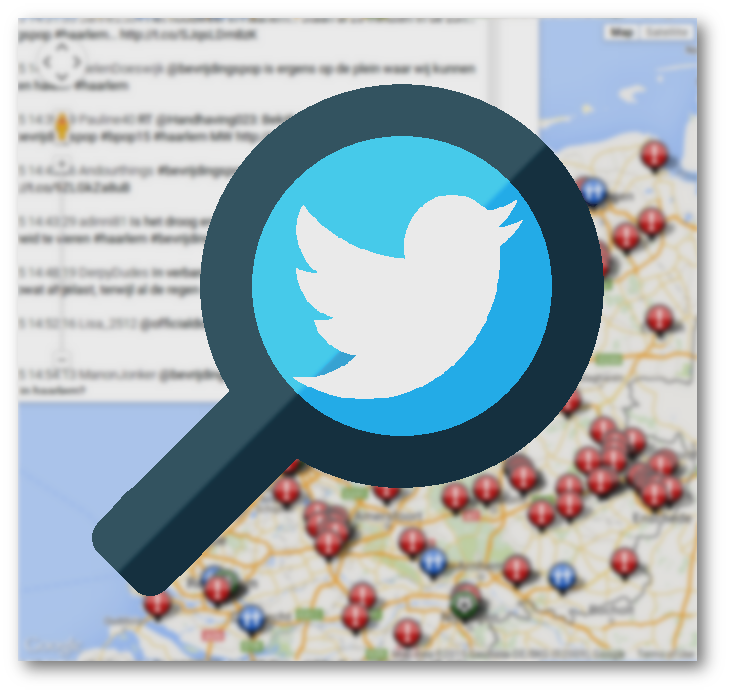
\includegraphics[scale=0.45]{mapchartlogo.png}
\vfill

%\vspace{0.8 cm}
%\hrule

\LARGE{\textsc{Bachelorscriptie Informatiekunde}}\\
\vspace{1.3 cm}
\Large{\textsc{\textbf{David de Kleer}}}
\vspace{0.5 cm}

\vrule
\hspace{0.2 cm}
\normalsize{\textsc{\today}}
\hspace{0.2 cm}
\vrule
\end{center}
\end{titlepage}
                              % genereert de titelpagina

%%%%%%%%%%%%%%%%%%%%%%%%%%%% HOOFDDOCUMENT

% table of contents op nieuwe pagina
\newpage
\tableofcontents

% nieuwe pagina voor voorwoord
\newpage
% phantomsection voor goede link in de table of contents, VOOR de sectie!
\phantomsection 
\s*{Voorwoord: Van orale traditie tot informatiesamenleving}
% toevoegen van s(ection)* aan inhoudsopgave moet in de sectie zelf!
\addcontentsline{toc}{section}{Voorwoord: Van orale traditie tot informatiesamenleving}
% Naamdicht dat ik een keer schreef in de trein omdat ik niks te doen had en
% nadacht over hoe ik mijn scriptie zou moeten beginnen
\begin{verse}
\it{\bf{O}p een stille zomernacht\\
    \bf{R}ond het vuur van het heden\\
    \bf{A}demt het verleden\\
    \bf{L}evend door de kracht\\
    \bf{E}n dynamiek, luid en zacht
\vl
    \bf{T}ongen van vuur\\
    \bf{R}oepend in het duister\\
    \bf{A}ls de strijd dan toch te heet wordt, is er\\
    \bf{D}e wind, die zachtjes fluistert\\
    \bf{I}n de kern van het verhaal\\
    \bf{T}ekenen van een wijze moraal, die\\
    \bf{I}n de harten blijft bestaan\\
    \bf{E}n nimmer zal vergaan}
\end{verse}

Mensen zijn inherent sociale wezens. Ze geven al eeuwenlang informatie aan 
elkaar door en doorstaan hierbij de tand des tijds door hun opgedane informatie 
op te slaan. Deze informatie is te zien als een erfenis waar volgende generaties 
op voort kunnen bouwen, een fundament voor het heden en de toekomst.
\vl
In de tijd dat er nog geen typemachines, recorders of computers bestonden moest 
er gebruik worden gemaakt van een primitieve, doch zeer effectieve manier van 
informatieoverdracht: de orale traditie. Deze traditie roept al snel een beeld 
op van oudere inwoners van stammen, die rond een knisperend vuur de jongeren 
lokale verhalen vol levenswijsheden vertelden. Dit mag misschien vrij primitief 
klinken, maar deze orale traditie vormt toch de basis van onze moderne 
samenleving, waarin we nog steeds onze kennis putten uit de informatiebronnen 
(gecreëerd vanuit de kennis van anderen) om ons heen. Daarbij zijn de manieren 
van doorgeven en opslaan van informatie door de eeuwen heen ontzettend vervormd, 
veranderd en vernieuwd, en kennen we een enorme hoeveelheden 
informatiedragers en daarmee methoden om informatie door te geven.
\vl
Er is wel een \it{maar}: Informatie heeft alleen waarde wanneer deze kan worden 
omgezet tot \it{kennis}. Het alleen maar opslaan van informatie betekent immers niet 
dat we die informatie automatisch tot ons nemen en omvormen tot kennis. Omdat 
onze hersenen een beperkte capaciteit hebben, kunnen we maar een beperkte 
hoeveelheid informatie in een keer verwerken. Informatiekunde kan helpen om 
grote hoeveelheden informatie inzichtelijker te maken en mensen tot nieuwe 
kennis en inzichten te brengen, door ze relevante informatie te bieden.
\vl
Het systeem dat wordt beschreven in deze bachelorscriptie Informatiekunde is een voorbeeld van het op 
overzichtelijke manier proberen te groeperen en weer te geven van relevante 
delen van een grote hoeveelheid informatie, gebaseerd op bepaalde kenmerken van 
deze informatie. 
\vl
Ik wil graag mijn scriptiebegeleiders – Johan Bos en Malvina Nissim – bedanken voor 
hun uitleg en begeleiding. Daarnaast wil ik Chris Pool bedanken voor zijn bijdrage
aan onze goede samenwerking. Mijn speciale dank gaat uit naar mijn ouders, vrienden, 
docenten en studiegenoten, voor hun steun, leerzame ervaringen en positieve contacten.
\vl
\it{David de Kleer, juni 2015}

% nieuwe pagina voor samenvatting
\newpage
\null\vspace{\fill}

\phantomsection
\s*{\hfill Samenvatting \hfill}
\addcontentsline{toc}{section}{Samenvatting}
Sociale media bieden een grote hoeveelheid informatie over de fysieke wereld, 
omdat mensen vertellen waar ze zijn, wat er in hun
omgeving gebeurt, of wat ze doen. Berichten van meerdere mensen op dezelfde
locatie kunnen worden gecombineerd tot mogelijke gebeurtenissen of \it{event candidates},
welke weer in categorie\"en zouden kunnen worden ingedeeld.
Hierdoor is het voor anderen in de buurt mogelijk om op de hoogte te blijven van wat er zoal
om hen heen gebeurt.
\vl
In deze scriptie presenteer ik een \it{state-of-the-art} benadering voor 
\it{event detection} – oftewel de detectie van gebeurtenissen of \it{events} – 
op Twitter. Hiervoor hebben we eerst
gebruik gemaakt van een methode voor \it{spatio-temporal clustering}, waarbij 
we verzamelde tweets (met locatie-informatie) clusteren binnen een bepaalde \it{GeoHash} (een locatie-representatie) en 
tijdsinterval. Vervolgens delen we met behulp van \it{supervised learning} event candidates op in de categorie\"en \ttt{geen\_event}, 
\ttt{sport}, \ttt{bijeenkomst}, \ttt{entertainment},
\ttt{incident} of \ttt{anders}. Hiervoor hebben we gebruik gemaakt van van twee
(\it{Naive Bayes}) \it{classifiers}, waarbij de eerste classifier alleen 
\it{word features}
gebruikt en de tweede features meer gerelateerd zijn aan 
\it{meta-informatie} van tweets.
Met name de eerste classifier blijkt behoorlijk goed te werken, deze behaalt 
alleen al een \it{accuracy} van 81\%. In combinatie met de tweede classifier
behalen we een accuracy van 84\%. Events worden gevisualiseerd met behulp
van een \it{Google Map interface} met \it{markers} en verrijkt met staafdiagrammen en
tweets zonder locatie-informatie.
\vspace{\fill}

% nieuwe pagina voor inleding
\newpage

\s{Inleiding}
Dankzij de opkomst van sociale media is er tegenwoordig een schat aan 
\it{real-time} informatie 
over de fysieke wereld te vinden op het Internet. Mensen zijn \it{sociale 
sensoren} (\citealt{sakaki2010earthquake}) geworden doordat ze
vertellen waar ze zijn, wat er in hun omgeving gebeurt, of wat ze doen. Sociale 
media bieden daardoor een metaforisch raam binnen
de digitale wereld, dat uitkijkt op onze fysieke wereld.
\vl
Op \it{Twitter} worden per dag miljoenen berichten (\it{tweets}) geplaatst, 
waarvan de nuttigheid voor andere gebruikers soms enigszins te
betwisten is (mensen vragen zich bijvoorbeeld af waarom plakken kaas twee 
centimeter groter zijn dan een boterham).
Het kan voor gebruikers handig zijn om via gefilterde Twitterdata inzicht te 
krijgen in wat er zoal om hen heen gebeurt: denk 
bijvoorbeeld aan journalisten of hulpdiensten, die hier altijd snel van op de 
hoogte moeten zijn. We willen een systeem bouwen dat 
voor Nederlandstalige tweets met locatie-informatie gebeurtenissen of \it{events} op Twitter op kan sporen (Event\it{Detective}) door tweets 
tot events te groeperen, oftewel 
een systeem voor \it{event detection} op Twitter.
We verstaan onder een event het
volgende: \it{``something non-trivially happening at a certain time or place''} 
(\citealt{yang1998study}), met daarbij als eis 
dat een event daadwerkelijk in de fysieke wereld plaatsvindt. 
Events moeten
tijdens de detectie worden gecategoriseerd (in bijvoorbeeld \ttt{sport} of \ttt{incident}), verrijkt met tweets zonder locatie-informatie (slechts 3\% van de 
tweets zijn voorzien van locatie-informatie (\citealt{leetaru2013mapping})) en vervolgens op een geschikte manier 
worden gevisualiseerd.
Het systeem detecteert geen \it{real-time events},
omdat we ons geheel willen richten op het proces van event detection en niet zozeer op real-time aspecten daarvan.
\vl
Ik zal in de Methode (hoofdstuk \ref{methode}) de implementatie van ons systeem 
beschrijven en in hoofdstuk \ref{resultaten} de experimenten, resultaten en evaluatie
presenteren. Daarna zal ik in hoofdstuk \ref{conclusie}, de Conclusie, ingaan op de 
hoofdvraag: \it{``Hoe kunnen we een systeem bouwen dat aan de hand van
Nederlandstalige tweets events kan detecteren, verrijken en visualiseren?''} Als 
eerste zal ik een link leggen met de wetenschap onderliggend aan
event detection in hoofdstuk \ref{theorie}, het Theoretisch Kader.

\s{Theoretisch kader}\label{theorie}

Het onderwerp van deze scriptie valt binnen de wetenschappelijke literatuur 
onder het thema \it{event detection} (in sociale media), waarbij dit thema op zijn beurt weer is in te 
passen binnen \it{Information Retrieval}. Volgens \citet{manning2008introduction} is Information 
Retrieval \it{“het vinden van ongestructureerd materiaal in grote 
informatiecollecties, waarbij dit materiaal tegemoet komt aan een 
informatiebehoefte”}. In event detection willen we binnen een grote collectie 
ongestructureerde data (in ons systeem gaat het om tweets) 
gebeurtenissen of \it{events} detecteren om mensen van events in de wereld op de 
hoogte te kunnen houden (de informatiebehoefte). 
\vl
De oorsprong van event detection is het door DARPA\footnote{Defense Advanced Research Projects Agency, het instituut voor onderzoek naar geavanceerde technologie van het Amerikaanse Ministerie van Defensie.} gesponsorde TDT-programma, 
oftewel \it{Topic Detection and Tracking} (\citealt{atefeh2013survey}). Het idee achter TDT was om 
de grote hoeveelheid informatie afkomstig uit verschillende 
nieuwsbronnen (in tekstvorm) op te delen in samenhangende nieuwsberichten, ontwikkelingen in 
reeds bestaande \it{news events} te detecteren en nieuwe news events te 
ontdekken ({\citealt{allan2002introduction}). Het TDT-programma bestond dus oorspronkelijk uit 
respectivelijk drie taken: de \it{segmentatie}, \it{detectie} en \it{opsporing} van events 
(\citealt{atefeh2013survey}). Het doel hiervan was om gebruikers inzicht te bieden in (de 
ontwikkeling van) nieuwe en interessante events die op de wereld 
plaatsvinden ({\citealt{allan2002introduction}).
\vl
Een systeem dat in staat is om event detection uit te voeren moet volgens 
TDT nieuwe of oudere, niet eerder ge\"identificeerde events kunnen ontdekken. 
Event detection kan voor TDT dus uit respectievelijk twee taken bestaan: \it{on-line} (dus 
\it{real-time}) \it{detection} en \it{retrospective detection} (\citealt{yang1998study}). Het systeem dat 
wordt beschreven in deze scriptie is niet real-time en valt dus onder retrospective detection, 
omdat we events in tweets uit het verleden willen ontdekken. Na enige aanpassing 
zou het mogelijk kunnen zijn om ons systeem ook on-line detection te laten uitvoeren, door te 
zorgen dat er constant input van de Twitter stream kan worden geanalyseerd. 
Hieruit blijkt dus dat een systeem voor event detection zowel een on-line als een retrospective 
component zou kunnen hebben.
\vl
Volgens \citet{atefeh2013survey} bestaat event detection uit drie hoofdprocessen: \it{``data 
preprocessing, data representation and data organization or clustering''}. \it{Data 
preprocessing} heeft alles te maken met de voorbereiding van ``rauwe'' data voordat 
deze door een systeem kan worden gebruikt (denk aan het filteren van 
stopwoorden, tokenisatie van tekst en het kiezen van goede datastructuren). 
\it{Data representation} gaat om het selecteren van voor event detection nuttige 
eigenschappen binnen de voorbereide data, bijvoorbeeld dat twee berichten binnen 
een bepaald tijdsinterval zijn gepubliceerd en qua inhoud op elkaar lijken. \it{Data 
organization} heeft betrekking op het daadwerkelijk indelen of organiseren van 
berichten in events, waarbij een systeem een model (gebaseerd op regels of 
\it{machine learning}\footnote{Binnen machine learning kunnen algoritmes worden 
gebruikt om patronen in een datarepresentatie te bepalen en aan de hand daarvan
data te classificeren.}) gebruikt om de gekozen datarepresentatie te organiseren. 
Deze eigenschappen kunnen soms vaker voorkomen: in ons systeem komt data organization
bijvoorbeeld drie keer voor (in \ref{ClusterCreator}, \ref{ClusterMerger} en \ref{ClassifierCreator}).
\vl
\citet{atefeh2013survey} geven aan dat het wat betreft de types events die kunnen worden 
gedetecteerd kan gaan om \it{specified} of \it{unspecified} events. Wanneer een systeem 
specified events detecteert, is het type event dat wordt gedetecteerd door het 
systeem bekend, of gaat het om een gepland event (\citealt{atefeh2013survey}). Voorbeelden 
uit de wetenschappelijke literatuur zijn systemen voor de detectie van 
aardbevingen (\citealt{sakaki2010earthquake}), concerten (\citealt{benson2011event}) en festivals (\citealt{lee2010measuring}). 
Wanneer het gaat om de detectie van unspecified events is het onbekend wat 
de events die we willen detecteren precies inhouden, of in gaan houden. Dit is 
het geval in bijvoorbeeld het laatste nieuws, denk aan een ongeval 
of een onderwerp dat onverwachts veel aandacht krijgt. Voorbeelden uit de 
wetenschappelijke literatuur zijn systemen voor de detectie van news events
(\citealt{sankaranarayanan2009twitterstand}), incidenten (\citealt{abel2012twitcident}), of algemene (ook kleinschalige) events die in de wereld
plaatsvinden (\citealt{walther2013geo}). Omdat we in ons systeem de laatstgenoemde
algemene events willen detecteren, richten we ons op de detectie van unspecified
events. Ik zal in de volgende alinea's wat dieper ingaan op de aanpak van de zojuist genoemde onderzoeken.
\vl
\citet{sakaki2010earthquake} willen aardbevingen en orkanen detecteren met behulp van Twitter en analyseren 
als eerste of hun verzamelde tweets hier daadwerkelijk over gaan. Ze gebruiken een \it{SVM} (\it{Support Vector Machine}, een machine learning algoritme
dat met name geschikt is voor binaire classificatie) om te bepalen of een tweet daadwerkelijk over
een natuurramp gaat die nu plaatsvindt (positieve klasse) of niet (negatieve klasse). De locatie
van positieve tweets wordt bepaald met behulp van \it{Kalman filtering}/\it{particle filtering}, waarmee de meest
waarschijnlijke locatie van een natuurramp uit de reeks (deels onbetrouwbare) locaties van Twitteraars kan worden gefilterd.
\vl
\citet{benson2011event} proberen Twitter in te zetten om muzikale events ontdekken die niet in andere media worden genoemd.
Ze maken gebruik van een (graaf)model (\it{factor graph model}) dat tweets analyseert, ze tot events clustert en bepaalt wat de waardes van eigenschappen van events (zoals artiest en locatie) zijn. Op het niveau van de tekst van tweets
wordt gebruik gemaakt van een \it{CRF} (\it{Conditional Random Field}, waarin een (graaf)model context/andere observaties kan gebruiken om labels aan input toe te kennen)
om de naam van een artiest of de locatie van een event uit geclusterde tweets te extraheren.
\vl
\citet{lee2010measuring} observeren voor de detectie van lokale festivals (in Japan) gedragspatronen van gebruikers met behulp
van tweets met locatie-informatie. Deze tweets worden op basis van hun co\"ordinaten met behulp van \it{K-means clustering}
geclusterd en ingedeeld in zogenaamde \it{ROIs} (\it{Regions of Interest}) in een \it{Voronoi}\footnote{De indeling van een vlak in subvlakken of regio's gebaseerd op punten die in dit vlak liggen.}-diagram. 
Binnen deze ROIs wordt met behulp van statistiek ``normaal'' en ``afwijkend'' gedrag van gebruikers vastgesteld. Een toename van gebruikers die een ROI binnenkomen of verlaten samen met een toenemend
aantal tweets blijkt een goede indicator voor lokale festivals te zijn.
\vl
\citet{sankaranarayanan2009twitterstand} willen tweets over het laatste nieuws kunnen opsporen. Ze
clusteren tweets (real-time) gebaseerd op tekstuele overeenkomst (\it{cosine similarity}) en verwijderen onbetrouwbare (\it{noisy}) tweets met behulp van een 
\it{Naive Bayes classifier}. Omdat noisy tweets een behoorlijk probleem vormden, is er ook gebruik gemaakt van \it{seeders}:
betrouwbare gebruikers die als eerste het laatste nieuws mogen rapporteren, wat betekent dat een bijbehorende cluster met reeds gevonden tweets zolang inactief
moet blijven. Een nadeel hiervan is wel dat het systeem door deze aanpak niet meteen het laatste nieuws kan detecteren, maar eerst moet wachten totdat een seeder hierover heeft bericht.
\vl
\citet{abel2012twitcident} richten zich op de detectie van tweets die incidenten rapporteren. Op basis van berichten van het P2000\footnote{P2000 geeft voor incidenten aan welk type incident er waar, wanneer en op welke schaal heeft plaatsgevonden.}
communicatiesysteem wordt er als eerste een incidentprofiel vastgesteld. Dit incidentprofiel bevat eigenschappen van een incident of
\it{facet:value}-paren (zoals \it{locatie:Moerdijk}). Met behulp van deze eigenschappen wordt een query gegenereerd die tweets teruggeeft die 
dergelijke eigenschappen bevatten, welke vervolgens semantisch worden verrijkt (met \it{NER}\footnote{\it{Named Entity Recognition}, de extractie van namen van bijvoorbeeld personen of locaties uit tekst.}, 
informatie afkomstig van links, tweet metadata en classificatie in onder andere tweets over slachtoffers of schade). De tweets die 
daadwerkelijk over een incident gaan moeten worden gefilterd, waarbij \it{semantic filtering} het beste bleek te werken: berichten die de
top k zwaarst wegende semantische eigenschappen bevatten blijven over.
\vl
Onze aanpak van event detection vertoont overeenkomsten met de aanpak van 
\citet{walther2013geo}. We gebruiken hetzelfde achterliggende idee: wanneer tweets 
binnen een bepaald tijdsinterval en op dezelfde locatie gepost
zijn, zou het goed kunnen dat ze een event bespreken: dit zijn mogelijke events of \it{event candidates}. 
\citet{walther2013geo} gebruiken daarnaast een aantal nuttige \it{features} (eigenschappen binnen de datarepresentatie) in 
hun event detection, waarop onze features zijn geïnspireerd. Wanneer we beschikking hebben over een
goede verzameling features (zoals een score voor de mate van overeenkomst van de inhoud van tweets), kunnen
we met behulp van geannoteerde data (event candidates voorzien van labels) \it{classifiers} trainen (bijvoorbeeld \it{Naive Bayes} of \it{SVM}). Deze classifiers kunnen
worden toegepast op nieuwe event candidates, om daaruit events te filteren. Onze classificiatie 
is in tegenstelling tot de classificatie van \citet{walther2013geo} niet \it{binair} (wel/geen event) maar \it{categorisch}, omdat we
events in categorieën (zoals \it{sport} of \it{bijeenkomst}) willen indelen. Daarnaast gebruiken we een andere 
locatie-representatie (geen radius rondom tweets, maar \it{GeoHash}\footnote{Zie 
figuur \ref{geohash} en de uitleg daarboven.}), en probeer ik events te verrijken met tweets zonder geo-informatie en 
Chris Pool met \it{named entity recognition}.

\s{Methode: Van data tot detective}\label{methode}

Nu volgt een beschrijving van de werking van ons systeem, van het verzamelen 
van de data tot de uiteindelijke detectie, verrijking en visualisatie van 
events (voor een \it{hands-on} benadering, zie listing \ref{commandos} in de bijlage (\ref{bijlage})). Het grootste gedeelte van deze processen wordt afgehandeld door een 
serie programma's in de programmeertaal Python, die in dit hoofdstuk behandeld 
zullen gaan worden. Wanneer er wordt verwezen naar een bestand (binnen een 
repository), is dit bestand te vinden in de git-repository 
\url{https://github.com/chrispool/Thesis/}. Als er geen uitleg over het gebruik 
van een programma wordt gegeven, is dit gewoon (onder \ttt{Unix}) uit te voeren als 
\ttt{./programmaNaam.py}. Ik zal ten eerste beschrijven hoe we aan \'e\'en van de 
meest fundamentele delen van ons systeem zijn gekomen: de data.

\ss{Verzamelen van data}\label{dataverzamelen}

We willen ons systeem trainen op retrospective data, dus op tweets uit het 
verleden. Onze tweet datasets (zie de map \ttt{corpus/} in de repository) zijn afkomstig van de Linuxserver \it{Karora}
(\ttt{karora.let.rug.nl}) van de Rijksuniversiteit Groningen. Deze server 
filtert constant 
(grotendeels) Nederlandstalige tweets uit de Twitter stream. De gefilterde 
tweets worden samen met hun metadata per uur in gecomprimeerde (\ttt{.out.gz}) 
bestanden in de map \ttt{/net/corpora/twitter2/\\Tweets} (op Karora) geplaatst. 
Met het volgende commando is het nu mogelijk om bijvoorbeeld de tweets 
(inclusief alle 
metadata) van 27 maart 2015, om 3 uur 's middags, te verkrijgen.
\begin{lstlisting}
$ zcat /net/corpora/twitter2/Tweets/2015/03/20150327:15.out.gz
\end{lstlisting}
\ttt{zcat} is identiek aan \ttt{gunzip -c}, dit betekent dat het bestand met 
tweets gedecomprimeerd wordt en de gedecomprimeerde tweet data wordt weggeschreven 
naar \ttt{standard output}.
\vl
Het programma \ttt{tweet2tab} (zie \ttt{scripts/tweet2tab} in de 
repository) is in 
staat om een aantal velden uit de zojuist verkregen gedecomprimeerde data te 
filteren en te scheiden met tabs, zodat deze velden eenvoudig door programma's
kunnen worden ingelezen. Voor ons systeem hebben we tweets nodig die beschikken 
over de velden:

\begin{bullets}
\item \ttt{text}: de tekst van de tweet
\item \ttt{coordinates}: breedte- en lengtegraad van de gebruiker toen de tweet 
werd
gepost
\item \ttt{user}: de naam van de gebruiker
\item \ttt{date}: datum en tijd
\end{bullets}

Om deze velden te verkrijgen kan het volgende commando worden toegepast op de 
output van het zojuist genoemde \ttt{zcat}-commando (op Karora):

\begin{lstlisting}
/net/corpora/twitter2/tools/tweet2tab -i text coordinates user date
\end{lstlisting}

Dit is in feite alle tweet data die we nodig hebben voor verdere verwerking. Er 
is alleen nog een probleem: \it{alle} tweets worden meegenomen in het vorige 
commando, niet alleen de tweets die voorzien zijn van een locatie! Het formaat 
van een tweet zonder locatie is (\ttt{<tab>} is het scheidingsteken):

\begin{lstlisting}
Kan niet slapen.<tab><tab>HOIIKBENMERLE<tab>2015-05-05 01:03:20 CEST Tue 
\end{lstlisting}

Er is dus nog een derde stap nodig om alleen de tweets met locatie te 
verkrijgen: de tweets die een leeg locatieveld hebben moeten worden 
overgeslagen. Dit kan zowel met een \ttt{grep}-commando als een klein script 
geschreven in Python (zie \ttt{scripts/get\_geotweets} in de repository):

\begin{bullets}
\item \ttt{grep}: Gebruik de Perl reguliere expressie (optie -P) 
\verb|^[^\t]+\t[^\t]+|. Deze reguliere expressie is waar wanneer er aan het 
begin van een regel 1 of meerdere keren een karakter staat dat geen tab is, 
vervolgens 1 keer een karakter dat wel een tab is en daarna weer 1 of meerdere 
keren een karakter dat geen tab is.
\item \ttt{get\_geotweets.py}: splitst alle regels in standard input op tabs en 
kijkt of 
het tweede element niet leeg is. De tweet wordt geprint naar \ttt{standard output} als dit het geval is.
\end{bullets}

Nu volgen twee voorbeeldcommando's die alle voorgaande handelingen combineren en laten zien 
hoe alle tweets van 27 maart op Karora kunnen worden verzameld in het bestand 
\ttt{march27.txt}.
\vl
Met \ttt{get\_geotweets.py}:
\begin{lstlisting}
$ zcat /net/corpora/twitter2/Tweets/2015/03/20150327???.out.gz | 
/net/corpora/twitter2/tools/tweet2tab -i text coordinates user date | 
python3 get_geotweets.py > march27.txt
\end{lstlisting}

Met \ttt{grep}:
\begin{lstlisting}
$ zcat /net/corpora/twitter2/Tweets/2015/03/20150327???.out.gz | 
/net/corpora/twitter2/tools/tweet2tab -i text coordinates user date | 
grep -P "^[^\t]+\t[^\t]+" > march27.txt
\end{lstlisting}

Het formaat van de verzamelde tweets is nu (\ttt{<tab>} is het scheidingsteken):
\begin{lstlisting}
Ik moet slapen	<tab>4.584649 51.854845<tab>tundraful<tab>2015-03-27 00:01:17 CET Fri 
\end{lstlisting}
\vspace*{-10pt}

\ss{\ttt{EventCandidates}: Generatie van event candidates}\label{EventCandidates}

Net als Walther, et al. willen we in ons systeem \it{event candidates} verzamelen: 
groepen of clusters van tweets die een gebeurtenis zouden kunnen zijn. Hiervoor 
groeperen we tweets die binnen een bepaalde tijd en plaats gepost zijn. We maken 
dus eigenlijk gebruik van \it{spatiotemporal clustering}: \it{“a process of grouping 
objects based on their spatial and temporal similarity”} (Kisilevich, et al.). 
\vl
Om event candidates te kunnen verzamelen is het van belang om eerst de 
verzamelde tweets en hun metadata om te zetten in een geschikte datastructuur in 
Python, de taak van de \ttt{Tweet\-Pre\-pro\-ces\-sor} (\ref{TweetPreprocessor}). Spatiotemporal clustering 
vindt in ons systeem plaats in twee stappen: de \ttt{ClusterCreator} (3.2.2) maakt 
clusters van tweets binnen een bepaalde locatie en een bepaald tijdsinterval, de 
\ttt{ClusterMerger} (3.2.3) voegt sommige gevonden clusters samen en selecteert event 
candidates.  Het idee achter de \ttt{ClusterCreator} en de \ttt{ClusterMerger} lijkt op het 
idee achter de \ttt{ClusterCreator} en de \ttt{ClusterUpdater} van Walther, et al.
\vl
Het programma \ttt{EventCandidates} accepteert als argumenten een bestand met tweets 
dat gegenereerd is door \'e\'en van de laatste twee commando's in sectie \ref{dataverzamelen}, en 
de naam van de dataset met event candidates die het programma moet generen.

\begin{lstlisting}
use: ./eventCandidates.py tweetfile datasetname
\end{lstlisting}
\vspace*{-10pt}

\sss{\ttt{TweetPreprocessor}: Tweets representeren in Python}\label{TweetPreprocessor}

We hebben ervoor gekozen om tweets op te slaan als Python \ttt{dictionaries} (in een 
\ttt{list}), waarvan de \ttt{keys} strings zijn en de \ttt{values} de verzamelde tweet (meta)data 
in de vorm van \ttt{strings} en \ttt{floats} voor de co\"ordinaten. Een \it{tweet dictionary} ziet er nu dus zo uit:

\begin{lstlisting}[language=Python]
tweetDict = {"text" : "tekst van tweet", "lon" : lengtegraad_float, "lat" : 
breedtegraad_float, "user" : "gebruikersnaam", "localTime" : "tijd in UTC"}
\end{lstlisting}

Het is belangrijk om in deze stap alvast na te denken over de volgende stap: hoe 
gaan we tweets clusteren op locatie en tijd, en wat is daarbij een handige en 
effici\"ente representatie van deze clusters? Hoe locatie- en tijdsdata in tweet 
dictionaries worden opgeslagen beïnvloedt immers hoe we deze data kunnen 
clusteren! 
\vl
De \bf{tijd} van tweets wordt standaard weergegeven als \ttt{"jaar-maand-dagnummer 
uur:minuut:se\-con\-de tijdszone dag"}. Wanneer uit deze string \ttt{"jaar-maand-dagnummer 
uur:minuut:se\-con\-de"} wordt gefilterd is het mogelijk tijd en datum met behulp van 
de Python \ttt{time}- en \ttt{datetime}-module in \bf{\it{Unix Time}} om te zetten, oftewel het aantal 
seconden dat is verstreken sinds 1 januari 1970. Hierdoor is het mogelijk om te 
rekenen met seconden wanneer tijden van tweets met elkaar vergeleken moeten 
worden, wat eenvoudiger is dan rekenen met een datum of tijd. Er kunnen direct 
wiskundige operatoren worden toegepast op tijden in Unix Time (omdat het 
integers zijn) en event candidates kunnen onder één enkel getal worden 
opgeslagen. Bezwaar tegen deze aanpak zou betrekking kunnen hebben op het geval 
wanneer tweets van twee verschillende events op dezelfde plaats op exact 
dezelfde seconde gepost worden. Wanneer dit het geval is, overschrijft één van 
beide events het andere event. Omdat dit waarschijnlijk niet vaak voor zal 
komen, nemen we dit risico.
\vl
De \bf{locatie} van tweets wordt standaard weergegeven als een co\"ordinaat (lengte- en 
breedtegraad). Een representatie van locatie-informatie waarin co\"ordinaten 
binnen hetzelfde gebied onder dezelfde identifier kunnen worden geplaatst is 
\bf{\it{GeoHash}}. Dit systeem deelt de wereld als het ware op in “hokjes” in een raster, 
waarbij een locatie dus niet meer bestaat uit een specifieke co\"ordinaat, maar 
uit een specifiek hokje (dat dus meerdere coordinaten omvat). Ieder hokje heeft 
een alfanumerieke code, waarbij de precisie van het hokje hoger wordt (en 
daarmee het betreffende gebied op aarde kleiner) wanneer de code langer is. 
Figuur \ref{geohash} geeft weer hoe dit ongeveer werkt.

\begin{figure}[H]
  \centering
    \image[width=0.6\textwidth]{geohash.png}
    \caption{GeoHash, de wereld binnen een raster}
  \label{geohash}
\end{figure}

We hebben gekozen om een GeoHash van precisie 7 (7 alfanumerieke karakters) te gebruiken. 
Hierbij is de grootte van de hokjes in het raster kleiner of gelijk aan 173x173 
meter\footnote{\url{http://www.movable-type.co.uk/scripts/geohash.html}}. We maken voor de omzetting van lengte- en breedtegraden naar GeoHashes 
gebruik van de Python-module \ttt{python-geohash}\footnote{\url{https://code.google.com/p/python-geohash/} (zie \ttt{modules/geohash.py} in de repository)}.
\vl
Nu het probleem van locatie en tijd is opgelost, is het handig om te kijken naar 
de \bf{tokenisatie} (of \bf{segmentatie} van de woorden) van de tekst van een tweet. Wanneer we bijvoorbeeld de tekst van 
tweets met elkaar willen vergelijken, komt het van pas om beschikking te hebben 
over een lijst met woordtokens die in deze tweets voorkomen. Om woordtokens te kunnen 
extraheren is het nodig om woordgrenzen te vinden. Daarvoor hebben we een simpele 
tokenizer geschreven, die gebaseerd is op de volgende reguliere expressie: 
\verb|[^a-zA-Z0-9#@]+|. Alle tekens in een string waarvoor niet geldt dat ze 1 of 
meerdere keren \ttt{a-z}, \ttt{A-9}, \ttt{0-9}, \ttt{\#}, of \ttt{@} bevatten, worden vervangen door een spatie 
(met behulp van \ttt{pattern.sub} in de {re}-module van Python). We hebben besloten om 
vóór het toepassen van de reguliere expressie links uit tweets te verwijderen 
(we willen puur te kijken naar de tekst). Wanneer er vervolgens een lijst van 
woorden zonder links overblijft, filteren we stopwoorden uit tweets met behulp 
van een lijst met stopwoorden. Deze lijst is samengesteld door de Nederlandse 
stopwoorden van de \ttt{nltk}-module\footnote{\url{http://www.nltk.org/}} van Python te combineren met een lijst van 
stopwoorden op internet (zie \ttt{corpus/stopwords.txt} in de repository).
\vl
Als we nu locatie, tijd en tokenisatie toevoegen aan het bestaande tweet 
dictionary, ziet deze er als volgt uit:

\begin{lstlisting}[language=Python]
tweetDict = {"text" : "tekst van tweet", "tokens" : "getokeniseerde tekst", 
"lon" : lengtegraad_float, "lat" : breedtegraad_float, "user" : "gebruikersnaam", 
"localTime" : "datum en tijd", "unixTime" : unixTime_int, "geoHash" : 
"GeoHash behorend bij lengte- en breedtegraad van tweet"}
\end{lstlisting}
\vspace*{-10pt}

\sss{\ttt{ClusterCreator}: Tweets clusteren op GeoHash en tijd}\label{ClusterCreator}

We moeten nu op basis van de gegenereerde tweet dictionaries tijd- en 
locatieclusters in een datastructuur zetten die we in het verdere systeem zullen 
gaan gebruiken. Omdat locaties met tijden gebruikt kunnen worden als (redelijk) 
unieke identifiers, zijn ze in combinatie geschikt als keys voor een dictionary. 
Er kunnen op verschillende tijden gebeurtenissen plaatsvinden binnen dezelfde 
locatie, dus is een logische en efficiënte representatie van clusters een 
dictionary met als keys de locaties (GeoHash) en als values dictionaries, met als 
keys tijden (Unix Time) en als value een lijst van tweet dictionaries.  
\vl
Merk hierbij op dat lijsten van tweet dictionaries binnen onze gekozen 
representatie clusters of \it{candidate clusters} zijn. Candidate clusters zijn 
clusters van tweets die binnen een bepaalde GeoHash en een bepaald tijdsinterval 
gepost zijn. Een candidate cluster kan blijven groeien in (tweet) omvang zolang 
dit cluster “in leven is”, wat betekent dat er een nieuwe tweet wordt gepost 
binnen de GeoHash en de tijd van de laatste tweet in een cluster + 60 minuten.
\vl
De structuur van een candidate cluster dictionary is dus als volgt:

\begin{lstlisting}[language=Python]
clusters = { "GeoHash 1" : { unixTimeLaatsteTweet_int : [ tweetDict1, ...], ...}, ...}
\end{lstlisting}
\vspace*{-10pt}

\sss{\ttt{ClusterMerger}: Clusters samenvoegen en event candidates selecteren}\label{ClusterMerger}

De clusters die we hebben verzameld vallen binnen een vrij klein gebied (kleiner 
of gelijk aan 173x173 meter), wat niet voldoende is voor events waarvan de 
deelnemers over grotere gebieden zijn verspreid. Daarom hebben we drie stappen 
aan het clusterproces toegevoegd die zorgen dat clusters worden samengevoegd met 
andere clusters in de buurt, wanneer ze qua locatie (\bf{stap 1}), tijd (\bf{stap 2}) en 
inhoud (\bf{stap 3}) overlappen. Dit werkt als volgt:

\begin{bullets}
\item \bf{Stap 1 - Overlap op locatie}: Omdat locaties bestaan uit GeoHashes of 
“hokjes”, is het mogelijk om voor deze hokjes te bepalen wat de “buurhokjes” 
zijn. Dit zijn de 8 hokjes die ieder hokje kunnen omringen (zie figuur \ref{geoneigh}). Buren 
van een GeoHash zijn eenvoudig te vinden door de \ttt{neigbors}-methode van de 
\ttt{geohash}-module te gebruiken: \ttt{geohash.neigbors(GeoHash)}.

\begin{figure}[H]
  \centering
    \image[width=0.4\textwidth]{geoneigh.png}
    \caption{Een GeoHash van precisie 5 met zijn 8 buren}
  \label{geoneigh}
\end{figure}

Een goede vraag om nu te stellen is: wanneer stop je met het kijken naar buren? 
Het is immers mogelijk om voor de buren van een GeoHash weer te kijken naar hun 
buren, voor die buren weer, etcetera... We hebben ervoor gekozen om maar \'e\'en 
keer de buren van een GeoHash op te zoeken, omdat een gebied van zo'n 400x400 
meter ons een goed formaat leek voor een gemiddeld event. 
\vl
We kunnen nu de clusters in alle buren (wanneer aanwezig) van een GeoHash 
bijlangs gaan om te kijken of ze qua tijd en inhoud overlappen met een cluster 
in de oorspronkelijke GeoHash.

\item \bf{Stap 2 - Overlap in tijd}: We kijken of clusters in tijd overlappen door de 
begin- en eindtijd van een cluster in de oorspronkelijke GeoHash met de begin- 
en eindtijden van clusters in een naburige GeoHash te vergelijken. Figuur \ref{overlap} laat 
zien hoe in slechts vier vergelijkingen te bepalen is of twee clusters in tijd 
overlappen.

\begin{figure}[H]
  \centering
    \image[width=0.65\textwidth]{overlap.png}
    \caption{Tijdsoverlap van twee clusters in vier vergelijkingen}
  \label{overlap}
\end{figure}

\item \textbf{Stap 3 – Overlap op inhoud}: Om te kunnen zien of twee clusters op inhoud 
overlappen bepalen we per cluster de 10 woorden met de hoogste \it{tf-idf score}. De 
tf-idf score wordt berekend door eerst te tellen hoe vaak een woord in een 
cluster voorkomt. Deze uitkomst wordt vermenigvuldigd met het logaritme van de 
totale hoeveelheid clusters, gedeeld door in hoeveel clusters een woord
voorkomt (\it{idf}, zie figuur \ref{idf}). idf is een compensatie voor woorden die vaak in 
veel documenten voorkomen, denk hierbij aan stopwoorden.

\begin{figure}[H]
  \centering
    \image[width=0.4\textwidth]{idf.png}
    \caption{Berekening van idf voor een term t in documenten D}
  \label{idf}
\end{figure}

\end{bullets}

Omdat na deze drie stappen de clusters zijn samengevoegd kunnen we nu event 
candidates gaan selecteren. Een samengevoegde cluster is in ons systeem een 
event candidate wanneer er minstens \bf{twee tweets} in staan van minstens \bf{twee 
gebruikers}. Deze event candidates worden door \ttt{EventCandidates} met behulp van de 
\ttt{json}-module\footnote{Met \ttt{json} kunnen datastructuren in Python eenvoudig 
in leesbaar formaat worden opgeslagen en later worden gebruikt door andere
programma's, zie \url{https://docs.python.org/3/library/json.html}.} opgeslagen
als \ttt{data/datasetnaam/Event\-Can\-di\-da\-tes.json}.
\vl
Het verschil tussen candidate clusters en event candidates is dus dat:

\begin{bullets}
\item \it{candidate clusters} (\ttt{ClusterCreator}) alleen aan de voorwaarde moeten voldoen 
dat ze tweets binnen dezelfde GeoHash en hetzelfde tijdsinterval bevatten
\item \it{event candidates} (\ttt{ClusterMerger}) kunnen \bf{bestaan} uit (samengevoegde) candidate 
clusters afkomstig uit een GeoHash \bf{en} zijn buren, waarbij een voorwaarde is dat 
ze minstens twee tweets en twee gebruikers bevatten
\end{bullets}

\ss{Annotatie van event candidates}\label{annotatie}

We willen events uit event candidates filteren met behulp van \it{supervised 
learning}. Binnen supervised learning is een leeralgoritme in staat om patronen 
vinden in \it{gelabelde} data, en op deze manier zelf in staat om labels aan nieuwe 
data toe te kennen. Om een leeralgoritme voor supervised learning toe te kunnen 
passen moeten we dus als eerste de door \ttt{EventCandidates} (\ref{EventCandidates}) gevonden event 
candidates voorzien van een label. Dit gebeurt met behulp van de \ttt{Annotator}
(\ref{Annotator}). We gebruiken de \ttt{Annotator} om allebei dezelfde dataset te annoteren, 
zodat we objectiever labels toe kunnen kennen aan event candidates. De evaluatie 
van onze annotatie en het opschonen van event candidates op basis van de 
evaluatie vindt plaats in \ttt{AnnotationEvaluation} (\ref{AnnotationEvaluation}).

\sss{\ttt{Annotator}: Interactieve annotatie van event candidates}\label{Annotator}

De annotatie van event candidates is een interactief proces. Eerst moet er een 
door \ttt{EventCan\-di\-da\-tes} gegenereerd dataset met event candidates worden ingelezen. 
Daarna worden alle event candidates één voor één weergegeven en kan een 
annotator voor iedere event candidate een label toekennen. We hebben besloten om 
event candidates niet binair te labelen (event/geen event), maar om categorieën 
aan ze toe te kennen. Het gaat hierbij om de volgende zes categorieën:

\begin{enumerate}
\item \ttt{geen\_event}: geen event
\item \ttt{sport}: events die betrekking hebben op sport
\item \ttt{entertainment}: concerten, festivals, theater, tv-shows...
\item \ttt{bijeenkomst}: bijeenkomsten van mensen rondom een bepaald (gespreks)motief
\item \ttt{incident}: ongelukken, branden, inbraken, vermissingen...
\item \ttt{anders}: event past niet in een andere categorie
\end{enumerate}

De datastructuur waarin annotaties worden opgeslagen lijkt erg veel op de 
datastructuur waarin event candidates zijn opgeslagen. In feite zijn de lijsten 
met tweet dictionaries vervangen door nummers van event types:

\begin{lstlisting}[language=Python]
clusters = {geoHash : { unixTimeLaatsteTweet_int : categorieNummer_int, ... }, ... }
\end{lstlisting}

De \ttt{Annotator} accepteert als argument de naam van een annotator, waardoor voor 
een \ttt{json}-bestand met annotaties (voor iedere annotator te vinden in 
\ttt{data/datasetnaam/an\-no\-ta\-ti\-on\_Name-judge.json}) kan worden ge\"identificeerd wie de 
annotator was, en annotaties op deze manier een unieke naam kunnen krijgen.

\begin{lstlisting}
use: Annotator.py Name-judge
\end{lstlisting}
\vspace*{-10pt}

\sss{\ttt{AnnotationEvaluation}: Annotatie evalueren en event candidates opschonen}\label{AnnotationEvaluation}

Omdat we event candidates door twee annotatoren laten annoteren, kunnen we voor 
annotaties de \it{interannotator agreement} bepalen – de mate waarin twee annotatoren 
het eens zijn – met behulp van de \it{Kappa-score}, zie figuur \ref{kappa}. Hierin staat $Pr(a)$ 
voor de hoeveelheid gevallen waarin annotatoren het met elkaar eens zijn en 
$Pr(e)$ voor de kans dat ze het eens zijn.

\begin{figure}[H]
  \centering
    \image[width=0.25\textwidth]{kappa.png}
    \caption{Berekening van de kappa-score}
  \label{kappa}
\end{figure}

\ttt{AnnotationEvaluation} vraagt als input een dataset met annotaties van twee 
annotatoren. Daarna bereiden we voor beide annotatoren twee lijsten voor, 
waarvan in lijst 1 de labels 0 t/m 5 (kappa-score voor categorie\"en) staan en in 
lijst 2 de labels 0 en 1 (kappa-score voor event of geen event). Deze lijsten 
staan voor beide annotatoren in dezelfde volgorde, waarna met behulp van een eigen 
implementatie de Kappa-score voor categorie\"en en event/geen event 
wordt berekend, met daarbij een \it{confusion matrix} voor categorieën en de 
\it{accuracy}. De laatste twee statistieken kunnen we enigszins vergelijken met de prestaties van 
ons systeem (als mensen het al in een bepaald percentage van de gevallen niet 
eens zijn, is het moeilijk om van een kunstmatig systeem te verwachten dat het 
deze gevallen goed identificeert).
\vl
Wanneer we het in onze annotatie oneens waren over de categorie van een event 
candidate wordt deze event candidate samen met de bijbehorende annotatie 
weggegooid. De overblijvende event candidates en annotaties worden in 
\ttt{data/datasetnaam/sanitizedEventCandidates.json} en 
\ttt{data/datasetnaam/sanitizedAnnotation.json} opgeslagen. Dit is onze \it{ground truth}, 
de \it{gold standard data} waaraan een leeralgoritme zich moet gaan aanpassen 
(\citealt{kobielus2014}).

\ss{Trainen van categorie en event classifiers}\label{train}

Omdat we met behulp van de annotatieprogramma's van sectie \ref{annotatie} train- en 
testdata kunnen annoteren, kunnen we na het annotatieproces \it{classifiers} gaan 
trainen. Een \it{classifier} is in supervised learning een functie die met behulp van 
een leeralgoritme automatisch klassen/labels toekent aan documenten, op basis 
van training op geannoteerde data (\citealt{manning2008introduction}). Om classifiers te kunnen 
genereren moeten we eerste een verzameling eigenschappen van event candidates 
identificeren. Daarin moeten onze classifiers patronen kunnen vinden die kunnnen 
helpen bij de identificatie van labels van (nieuwe) event candidates. Om deze 
reden moet de verzameling eigenschappen waarop we de classifiers trainen dus 
worden geëxtraheerd uit alle event candidates waarop we onze classifiers willen 
toepassen. De extractie van deze eigenschappen of features is de taak van de 
\ttt{FeatureSelector} (\ref{FeatureSelector}). Het daadwerkelijke trainen, testen en evalueren van 
classifiers gebaseerd op verschillende leeralgoritmen vindt plaats in de 
\ttt{ClassifierCreator} (\ref{ClassifierCreator}).

\sss{\ttt{FeatureSelector}: Extractie van features uit event candidates}\label{FeatureSelector}

Als we willen dat onze classifiers goed presteren, is het van belang om een 
nuttige verzameling features van event candidates te bepalen. We hebben voor 
onze experimenten 9 features ge\"identificeerd:

\begin{bullets}
\item \ttt{wordOverlapUser}: Berekent de overlap van woorden tussen gebruikers binnen een 
event candidate, waarbij de score hoger wordt wanneer overlappende woorden een 
hoge df-waarde hebben. In hoe meer documenten per gebruiker (tweets) een woord staat, des 
te hoger de score wordt, waarbij hashtags een bonus krijgen omdat ze een 
gemeenschappelijk thema of onderwerp aan kunnen geven. De score wordt 
vermenigvuldigd met de hoeveelheid gebruikers, gedeeld door de hoeveelheid 
tweets binnen de event candidate, en afgerond op 0.5 zodat de kans op overlap 
met andere event candidates groter is.
\item \ttt{wordOverlapSimple}: Simpele score voor woordoverlap. De hoeveelheid woorden die 
overlappen voor elke tweet binnen een event candidate (hashtags krijgen wederom 
een bonus) wordt gedeeld door de hoeveelheid tweets binnen deze event candidate 
en afgerond op 0.5.
\item \ttt{wordOverlap}: Lijkt vrij veel op \ttt{wordOverlapSimple}, het verschil is dat de 
overlaptellingen van woorden worden vermenigvuldigd met de idf-scores van deze 
woorden binnen een event candidate.
\item \ttt{location}: De gemiddelde locatie van de gebruikers in een event candidate wordt 
bepaald door het (\it{Cartesisiaans}\footnote{Officieel moet er bij berekening van 
een gemiddelde coördinaat rekening worden gehouden met de
kromming van het aardoppervlak, anders ontstaat er een afwijking in het 
uiteindelijke coördinaat. Omdat het bij een event candidate gaat om een klein 
vlak op aarde zal de afwijking van dit coördinaat waarschijnlijk niet zo groot 
zijn. Daarom berekenen we gewoon het “standaard” gemiddelde van de coördinaten, net 
alsof ze punten in een Cartesiaans coördinatenstelsel zijn: een platte aarde!}) 
gemiddelde van de lengte- en breedtegraden van de tweets binnen de event 
candidate te berekenen. Dit gemiddelde coördinaat wordt omgezet naar een GeoHash van 
precisie 6 met behulp van de \ttt{geohash}-module: \ttt{geohash.encode(breed\-te\-graad, 
lengtegraad, precisie)}.
\item \ttt{uniqueUsers}: De hoeveelheid unieke gebruikers binnen een event candidate.
\item \ttt{nTweets}: De hoeveelheid tweets binnen een event candidate.
\item \ttt{wordFeatures}: Binaire features die aangeven of de top n woorden met de hoogste 
tf-idf score wel of niet in een event candidate voorkomen. Deze word features 
gebruiken we om een classifier voor event candidate categorieën (\it{category 
classifier}) te trainen.
\item \ttt{category}: In welke categorie een getrainde category classifier een event 
candidate indeelt.
\end{bullets}

Wanneer een programma de features uit een event candidate wil extraheren, is het 
mogelijk om \ttt{getFeatures(candidate, features)} te gebruiken. \ttt{candidate} is hierin 
een event candidate, \ttt{features} is een lijst van de zojuist genoemde features in 
de vorm van strings. Deze methode levert een dictionary op, met als keys de namen 
van features en als values de waarden van deze features voor een event 
candidate.

\sss{\ttt{ClassifierCreator}: Training en evaluatie van classifiers}\label{ClassifierCreator}

Om classifiers te kunnen trainen moeten eerst de geannoteerde data en 
bijbehorende event candidates worden ingelezen in een geschikte representatie. 
Welke data precies wordt ingelezen hangt af van de \it{modus} waarin de 
ClassifierCreator wordt gebruikt. Er zijn twee modi, namelijk \bf{DEVTEST} en \bf{TEST}:

\begin{bullets}
\item \bf{DEVTEST modus}: De input bestaat uit één enkel geannoteerd dataset. Deze 
dataset wordt opgesplitst door een willekeurige \it{80/20 split} (80\% traindata en 
20\% testdata) toe te passen. De DEVTEST modus doorloopt tien iteraties waarin 
classifiers worden getraind en geëvalueerd op de willekeurig opgesplitste testdata: \it{cross-validation}.

\item \bf{TEST modus}: De input bestaat uit twee geannoteerde datasets, namelijk een 
train- en een testdataset. Deze modus doorloopt één iteratie, waarbij 
classifiers getraind kunnen worden op de gehele dataset van de DEVTEST modus en 
getest op een nieuwe dataset die ons programma nooit eerder heeft “gezien”. 
Features kunnen voor een DEVTEST namelijk helemaal worden geoptimaliseerd, 
waarbij de keuze van features misschien helemaal niet geschikt is voor 
toepassing op een nieuwe dataset: dit komt naar voren in de “echte” test. Dit 
geeft een eerlijkere indicatie van de prestaties van het systeem.
\end{bullets}

De train- en testdata worden in het programma opgeslagen als een lijst van 
tuples, waarbij de tuples bestaan uit een event candidate (herinnering: dit was 
een lijst van tweet dictionaries) en het bijbehorende label afkomstig van de 
annotaties. De structuur is dus als volgt:

\begin{lstlisting}[language=Python]
dataset = [ ([{"text" : "tweet text", ...}, ...], "bijbehorend label"), ...]
\end{lstlisting}

Nu de train- en testdata in een geschikte representatie zijn opgeslagen, kunnen 
we classifiers trainen. We hebben ervoor gekozen om gebruik te maken van twee 
classifiers in ons systeem:

\begin{bullets}
\item \ttt{categoryClassifier}: De eerste classifier die het systeem traint probeert op 
basis van woorden in een event candidate de categorie (zie \ref{Annotator} voor de labels) 
van een event candidate te achterhalen. Voor de training extraheren we eerst de 
\ttt{wordFeatures} (\ref{FeatureSelector}) uit de train- en testdata. Features hebben de volgende 
structuur:

\begin{lstlisting}[language=Python]
features = [( {"wordFeatures": ["word1" : False, ...]}, "bijbehorend label"), ...]
\end{lstlisting}

De \ttt{nltk}-module kan classifiers trainen met dergelijke lijsten van \ttt{tuples} met 
\ttt{feature dictionaries} en labels. De classifier die we voor categorie\"en gebruiken 
is een \it{Naive Bayes} classifier van de python-module \ttt{scikit-learn}\footnote{\url{http://scikit-learn.org}}, die kan worden 
getraind met behulp van een eenvoudige wrapper van de \ttt{nltk}-module: 
\ttt{SklearnClassifier}. Deze wrapper kan worden gebruikt om \ttt{scikit-learn} classifiers 
te trainen die data in hetzelfde formaat als \ttt{nltk}-classifiers accepteren. De 
reden dat we niet de standaard Naive Bayes implementatie van \ttt{nltk} gebruiken is 
dat de implementatie van \ttt{scikit-learn} sneller blijkt te werken en vrijwel 
identieke resultaten oplevert.
\item \ttt{eventClassifier}: Voor de tweede classifier extraheren we wederom features 
(\ref{FeatureSelector}) uit event candidates, die op dezelfde manier worden opgeslagen als voor 
de eerste classifier. De \ttt{eventClassifier} gebruikt de door de \ttt{categoryClassifier} 
toegekende labels met daarbij andere features (zoals \ttt{wordOverlapUser} of 
\ttt{location}) om nogmaals te bepalen onder welke categorie een event thuishoort. We 
hebben besloten om voor deze classifier te kiezen voor de Naive Bayes classifier 
van \ttt{nltk}.
\end{bullets}

De \ttt{categoryClassifier} is te zien als een soort basisclassifier die alleen \it{word 
features} gebruikt om event candidates in categorie\"en in te delen. De 
\ttt{eventClassifier} past \it{finetuning} toe op de categorielabels van de 
\ttt{categoryClassifier}, met behulp van features die meer betrekking hebben op de 
\it{metadata} van event candidates. We willen hiermee een conceptuele scheiding aangeven.
\vl
Wanneer beide classifiers zijn getraind berekent het programma een aantal 
statistieken voor de evaluatie. Deze statistieken omvatten de \it{precision}, \it{recall}, 
\it{f-score}, \it{accuracy} en \it{confusion matrix} voor iedere training van de classifiers 
(iteratie). De statistieken worden met behulp van de \ttt{metrics} van \ttt{nltk} bepaald en 
een aantal daarvan met behulp van de \ttt{tabulate}-module (\ttt{zie modules/tabulate.py}) 
in een tabel gezet.
\vl
Als het programma in de TEST modus wordt uitgevoerd worden de (laatst) getrainde 
classifiers opgeslagen als binaire bestanden in 
\ttt{data/datasetnaam/eventClassifier.bin} en \ttt{data/da\-ta\-set\-naam/categoryClassifier.bin}, 
met behulp van de pickle-module\footnote{\url{https://docs.python.org/3/library/pickle.html}}.
\ttt{pickle} is vergelijkbaar met \ttt{json}, alleen worden bestanden in binair in plaats van
leesbaar formaat opgeslagen. Het doel van beide modules is gelijkwaardig, namelijk
\it{serialisatie}\footnote{Objecten of datastructuren opslaan zodat ze later weer kunnen 
worden opgebouwd.}.

\ss{Detectie, verrijking en visualisatie van events}\label{detect}

De in \ref{train} getrainde classifiers kunnen nu worden toegepast om events te 
detecteren op basis van nieuwe event candidates. Dit is het proces dat het aan 
ons systeem gelijknamige (hoofd)programma \ttt{EventDetective} (3.5.1) uitvoert. De 
verrijking van events door middel van tweets zonder geo-informatie vindt plaats 
in \ttt{EventDetectiveChart} (3.5.2). De bestanden in de map \ttt{/vis/map} (3.5.3) handelen 
de visualisatie van events af. \ttt{EventDetective} en \ttt{EventDetectiveChart} hebben een 
visualisatiecomponent (\ttt{generateMarkers}, zie 3.5.3) omdat ze de input voor de 
visualisatie moeten geven.

\sss{\ttt{EventDetective}: Detectie van events}\label{EventDetective}

De naam \ttt{EventDetective} is afkomstig van event detection, het centrale thema van 
het onderzoek onderliggend aan het onderwerp van deze scriptie, en een soort 
\it{``detective-metafoor''}. Een detective (\it{classifier}) krijgt vaak een grote 
hoeveelheid bewijsmateriaal (\it{event candidates met geëxtraheerde features}) waaruit 
hij moet bepalen welke bewijzen leiden naar de juiste conclusie, de oorzaak van 
het misdrijf (\it{of een event candidate wel of geen event is}).
\vl
Om events te kunnen detecteren vereist de \ttt{EventDetective} als input eerst een 
dataset met classifiers en vervolgens een dataset met nieuwe event candidates, 
waarin events moeten worden gedetecteerd.  
Vervolgens wordt de FeatureSelector (\ref{FeatureSelector}) toegepast om features voor de \ttt{category-} 
en de \ttt{eventClassifier} uit de nieuwe event candidates te halen. Beide 
classifiers bepalen daarna een categorielabel voor de event candidates. Wanneer 
ze onder een categorie vallen die niet gelijk is aan \ttt{geen\_event} worden ze aan 
een lijst met events toegevoegd.

\sss{\ttt{EventDetectiveChart}: Verrijking van events}\label{EventDetectiveChart}

\ttt{EventDetectiveChart} erft over van \ttt{EventDetective} en bevat qua detectie van 
events dezelfde functionaliteit. De extra stap die in dit programma plaatsvindt 
is de toevoeging van tweets zonder geo-informatie. Omdat er niet meer zoveel 
tijd was voor een uitgebreide extra componenent heb ik voor deze stap een \it{Proof 
of Concept} of versimpeld prototype ontwikkeld.
\vl
Het is van belang dat tweets zonder geo-informatie vóór volledige processing met 
behulp van \it{heuristieken} kunnen worden gescand op overeenkomst met een event, 
omdat we hiervoor \it{alle} Nederlandse tweets in een periode moeten scannen. Op \bf{de 
dag} 5 mei 2015 zijn er bijvoorbeeld 760000 tweets gepost (100 MB), waarbij de 
hoeveelheid tweets met geo-informatie over \bf{de hele maand} maart ter vergelijking ongeveer 570000 
tweets (79 MB) bedraagt. Wanneer een maand aan tweets zonder geo-informatie moet 
worden gescand, gaat het al gauw om ongeveer 10 GB(!) aan tweets.
\vl
Een schaalbare benadering van dit probleem is om eerst de belangrijkste woorden 
uit een event te verzamelen. Onder belangrijke woorden versta ik simpelweg de n 
woorden met de hoogste \it{df-waarden} (in hoeveel tweets een woord voorkomt) binnen 
een event, waarbij termen met hashtags (belangrijk) dubbel worden geteld. Vervolgens
kunnen steeds alle tweets binnen het tijdsinterval van een event worden ingelezen 
(bijvoorbeeld de tweets van die dag of van de uren waarin het event nog ``in leven
was''). In een echte toepassing is het van belang dat ingelezen tweets na 
verwerking steeds worden uitgelezen om te voorkomen dat het geheugen helemaal volloopt. 
\vl
Een eenvoudige heuristiek die aangeeft dat tweets verder moeten worden verwerkt 
is wanneer ze twee van de top drie woorden uit de lijst van woorden met de 
hoogste df-waarden van een event bevatten. Een woord uit die top drie mag in een 
tweet voorkomen als \ttt{"\ woord"} (let op de spatie!), \ttt{"@woord"} of \ttt{"\#woord"}. Op deze 
manier is het zelfs niet eens nodig om de velden van de tweet te splitsen om ze 
apart in te kunnen lezen. De velden van tweets die genoeg woorden bevatten om 
verder te worden verwerkt worden wel gesplitst en in een tweet dictionary gezet. 
Hiervoor was een aanpassing aan de \ttt{TweetPreprocessor} (\ref{TweetPreprocessor}) nodig, omdat de 
tweet data zonder geo-informatie het veld voor locatie mist. Eventuele stappen 
die hierna nog plaats zouden kunnen vinden is het berekenen van een \it{similarity 
score} met de tweets in een event, maar hier ben ik verder niet meer aan 
toegekomen.

\sss{\ttt{generateMarkers} en \ttt{vis/map/}: Visualisatie van events}\label{eventvis}

Om events te visualiseren en de resultaten van ons systeem te kunnen presenteren 
hebben we gebruik gemaakt van \it{markers} met een \ttt{InfoWindow} op een \it{Google Map}, zie 
figuur \ref{mapmarker}.

\begin{figure}[H]
  \centering
    \image[width=0.5\textwidth]{mapmarker.png}
    \caption{Voorbeeld van een Google Map Marker met een InfoWindow}
  \label{mapmarker}
\end{figure}

De inhoud van het \ttt{InfoWindow} bestaat uit \it{de tweets die horen bij een event, 
samen met hun metadata (tijd, gebruiker, locatie)}, in chronologische volgorde. 
Om de coordinaten van een marker te bepalen maken we net als voor de 
\ttt{location}-feature (\ref{FeatureSelector}) gebruik van het \it{Cartesiaans gemiddelde van de lengte- 
en breedtegraden} van de tweets binnen een cluster. We hebben de \it{categorie} van 
een event nodig omdat we voor elke categorie een uniek icoon willen gebruiken, 
zodat gelijk aan een marker te identificeren is om welk type event het gaat (zie 
figuur \ref{markers}). Al deze data wordt door de \ttt{EventDetective} (\ref{EventDetective}) in \ttt{generateMarkers} 
opgeslagen als een variabele in een Javascriptbestand (\ttt{vis/map/js/markers.js}) 
met het formaat:

% eigenlijk niet Python, maar dit werkt ook prima
\begin{lstlisting}[language=Python]
locations = [['tweet tekst/metadata', gemBreedtegraad_float, gemLengtegraad_float, 
'categorielabel'], ...] 
\end{lstlisting}

Elke lijst binnen deze \ttt{locations}-lijst is een event dat met behulp van 
\ttt{vis/map/map.html} kan worden gevisualiseerd. De werking van \ttt{vis/map/map.html} is 
vrij vanzelfsprekend, er wordt een Google Map gemaakt met behulp van de Google 
Maps API en markers (met iconen per categorie) worden gegenereerd aan de hand 
van de lijsten in \ttt{locations}.

\begin{figure}[H]
  \centering
    \image[width=0.6\textwidth]{markers.png}
    \caption{Marker iconen: entertainment, incident, bijeenkomst, anders, sport}
  \label{markers}
\end{figure}

Naast de standaard visualisatie heb ik nog een extra visualisatie-optie aan het systeem 
toegevoegd: een Google Map met staafdiagram, met behulp van het \it{jQuery framework} van 
\ttt{High\-Charts}\footnote{\url{http://www.highcharts.com/products/highcharts}}. 
Het idee hierachter is als volgt: wanneer events worden verrijkt 
met tweets zonder geo-informatie, en er wordt bijvoorbeeld een belangrijke 
voetbalwedstrijd gevonden is het makkelijk om overspoeld te raken door de 
hoeveelheid tweets bij een dergelijk event. Daarom leek het me handig om tweets te 
groeperen per twee minuten\footnote{Dit is mogelijk door de Unix Time van tweets 
te delen door 120, af te ronden en weer vermenigvuldigen met 120. Deze afgeronde 
Unix Times kunnen als keys in een dictionary met als values lijsten van tweet 
dictionaries worden gebruikt om tweets op twee minuten te groeperen.} en in een 
staafdiagram te laten zien, waarbij maximaal 10 tweets uit die periode worden 
weergegeven wanneer de muiscursor op een staaf wordt gezet. Op deze manier is 
het eenvoudig om trends in grote hoeveelheden tweets te ontdekken.
\vl
\ttt{EventDetectiveChart} genereert met behulp van zijn (\it{overridden}) \ttt{generateMarkers} 
dezelfde data als de \ttt{EventDetective}, met daarbij als toevoeging de \it{x- en 
y-coordinaten} ($x$ is de tijd, $y$ de hoeveelheid tweets binnen twee minuten) van 
het staafdiagram, de \it{titel van het event} in de vorm van de drie woorden met de 
hoogste df-waarden en de \it{ondertitel} in de vorm van de dag waarop het event 
plaatsvond. De in \ref{EventDetectiveChart} gevonden tweets zonder locatie-informatie worden 
\bf{dikgedrukt} weergegeven in de \ttt{InfoWindow}s bij markers op de kaart. De structuur 
van de eerder genoemde \ttt{locations}-lijst is afgezien van de toevoeging van deze 
data precies hetzelfde.
\vl
De visualisatie van events met hun bijbehorende staafdiagrammen vindt plaats in 
\ttt{vis/map/\\map\_chart.html}. Het verschil met \ttt{vis/map/chart.html} is dat de pagina nu 
in twee delen wordt verdeeld, waarbij aan de linkerkant de Google Map met 
markers wordt weergegeven en aan de rechterkant de \ttt{HighCharts}-grafiek die hoort 
bij een aangeklikte marker.

\s{Experimenten, resultaten en evaluatie}\label{resultaten}

Ik zal nu de met onze \ttt{EventDetective}-software uitgevoerde experimenten – inclusief verkregen resultaten 
en evaluatie – beschrijven.

\ss{Data verzamelen event candidates genereren}

Voor onze gezamenlijke event detection experimenten hebben we gebruik gemaakt van 
twee geannoteerde datasets (om te trainen en te testen, zie de TEST-modus in \ref{ClassifierCreator}).
De dataset waarop we hebben getraind bestaat uit alle 566549 tweets met geo-informatie van
maart 2015 (\ttt{/corpus/march.txt}). Onze testset bestaat uit de 165848 tweets met geo-informatie
van de tweede helft van april 2015 (\ttt{/corpus/april.txt}). Beide datasets zijn verzameld zoals is beschreven in
\ref{dataverzamelen}. We hebben \ttt{EventCandidates} (\ref{EventCandidates}) gebruikt om de event 
candidates uit beide datasets te extraheren (zie \ttt{data/dataset/EventCandidates.json} voor de trainset en 
\ttt{data/testset/EventCandidates.json} voor de testset).

\ss{Het annotatieproces}

We hebben voor onze train- en testset allebei met behulp van de \ttt{Annotator} (\ref{Annotator})
respectievelijk 1350 en 500 event candidates geannoteerd. Vervolgens heeft \ttt{AnnotationEvaluation} (\ref{AnnotationEvaluation}) 
de kappa-score en de confusion matrices van onze annotaties bepaald, zie tabel \ref{annotationtrain} en \ref{annotationtest}.
Bij elke confusion matrix worden de kappa-score voor categorie\"en (\it{categoryKappa}), event/geen event (\it{eventKappa}) en
de \it{accuracy} (hoe vaak we het eens waren) gegeven.

\begin{table}[H]
\centering
\caption{Trainset - categoryKappa: 0.79, eventKappa: 0.8, accuracy: 0.868}\label{annotationtrain}
\vspace*{-5pt}
\begin{tabular}{lcccccc}
& \multicolumn{1}{l}{\textbf{anders}} & \multicolumn{1}{l}{\textbf{bijeenk}} & \multicolumn{1}{l}{\textbf{entertain}} & \multicolumn{1}{l}{\textbf{geen\_event}} & \multicolumn{1}{l}{\textbf{incident}} & \multicolumn{1}{l}{\textbf{sport}} \\ \cline{2-7} 
\multicolumn{1}{l|}{\textbf{anders}} & \multicolumn{1}{c|}{\textless1\textgreater} & \multicolumn{1}{c|}{.} & \multicolumn{1}{c|}{.} & \multicolumn{1}{c|}{2} & \multicolumn{1}{c|}{1} & \multicolumn{1}{c|}{1} \\ \cline{2-7} 
\multicolumn{1}{l|}{\textbf{bijeenk}} & \multicolumn{1}{c|}{21} & \multicolumn{1}{c|}{\textless207\textgreater} & \multicolumn{1}{c|}{7} & \multicolumn{1}{c|}{25} & \multicolumn{1}{c|}{.} & \multicolumn{1}{c|}{2} \\ \cline{2-7} 
\multicolumn{1}{l|}{\textbf{entertain}} & \multicolumn{1}{c|}{3} & \multicolumn{1}{c|}{.} & \multicolumn{1}{c|}{\textless20\textgreater} & \multicolumn{1}{c|}{5} & \multicolumn{1}{c|}{.} & \multicolumn{1}{c|}{.} \\ \cline{2-7} 
\multicolumn{1}{l|}{\textbf{geen\_event}} & \multicolumn{1}{c|}{14} & \multicolumn{1}{c|}{27} & \multicolumn{1}{c|}{18} & \multicolumn{1}{c|}{\textless619\textgreater} & \multicolumn{1}{c|}{9} & \multicolumn{1}{c|}{9} \\ \cline{2-7} 
\multicolumn{1}{l|}{\textbf{incident}} & \multicolumn{1}{c|}{1} & \multicolumn{1}{c|}{2} & \multicolumn{1}{c|}{.} & \multicolumn{1}{c|}{12} & \multicolumn{1}{c|}{\textless178\textgreater} & \multicolumn{1}{c|}{.} \\ \cline{2-7} 
\multicolumn{1}{l|}{\textbf{sport}} & \multicolumn{1}{c|}{1} & \multicolumn{1}{c|}{.} & \multicolumn{1}{c|}{.} & \multicolumn{1}{c|}{5} & \multicolumn{1}{c|}{.} & \multicolumn{1}{c|}{\textless60\textgreater} \\ \cline{2-7} 
\end{tabular}
\end{table}

\begin{table}[H]
\centering
\caption{Testset - categoryKappa: 0.82, eventKappa: 0.8, accuracy: 0.86}\label{annotationtest}
\vspace*{-5pt}
\begin{tabular}{lcccccc}
& \multicolumn{1}{l}{\textbf{anders}}            & \multicolumn{1}{l}{\textbf{bijeenk}}              & \multicolumn{1}{l}{\textbf{entertain}}            & \multicolumn{1}{l}{\textbf{geen\_event}}              & \multicolumn{1}{l}{\textbf{incident}}             & \multicolumn{1}{l}{\textbf{sport}}    \\ \cline{2-7} 
\multicolumn{1}{l|}{\textbf{anders}} & \multicolumn{1}{c|}{\textless.\textgreater} & \multicolumn{1}{c|}{.}                        & \multicolumn{1}{c|}{.}                      & \multicolumn{1}{c|}{.}                        & \multicolumn{1}{c|}{1}                       & \multicolumn{1}{c|}{.}              \\ \cline{2-7} 
\multicolumn{1}{l|}{\textbf{bijeenk}} & \multicolumn{1}{c|}{4}                      & \multicolumn{1}{c|}{\textless110\textgreater} & \multicolumn{1}{c|}{13}                     & \multicolumn{1}{c|}{9}                        & \multicolumn{1}{c|}{.}                       & \multicolumn{1}{c|}{3}              \\ \cline{2-7} 
\multicolumn{1}{l|}{\textbf{entertain}} & \multicolumn{1}{c|}{.}                      & \multicolumn{1}{c|}{.}                        & \multicolumn{1}{c|}{\textless8\textgreater} & \multicolumn{1}{c|}{2}                        & \multicolumn{1}{c|}{.}                       & \multicolumn{1}{c|}{.}              \\ \cline{2-7} 
\multicolumn{1}{l|}{\textbf{geen\_event}} & \multicolumn{1}{c|}{3}                      & \multicolumn{1}{c|}{19}                       & \multicolumn{1}{c|}{4}                      & \multicolumn{1}{c|}{\textless199\textgreater} & \multicolumn{1}{c|}{4}                       & \multicolumn{1}{c|}{2}              \\ \cline{2-7} 
\multicolumn{1}{l|}{\textbf{incident}} & \multicolumn{1}{c|}{1}                      & \multicolumn{1}{c|}{.}                        & \multicolumn{1}{c|}{.}                      & \multicolumn{1}{c|}{.}                        & \multicolumn{1}{c|}{\textless78\textgreater} & \multicolumn{1}{c|}{.}              \\ \cline{2-7} 
\multicolumn{1}{l|}{\textbf{sport}} & \multicolumn{1}{c|}{.}                      & \multicolumn{1}{c|}{1}                        & \multicolumn{1}{c|}{2}                      & \multicolumn{1}{c|}{2}                        & \multicolumn{1}{c|}{.}                       & \multicolumn{1}{c|}{\textless60\textgreater} \\ \cline{2-7} 
\end{tabular}
\end{table}

We hebben dus voor zowel train- als testset kappa-scores van 0.8 behaald. Volgens \citet{manning2008introduction} is 
een agreement boven de 0.8 ``goed'', dus we kunnen zeggen dat er hier sprake is van een behoorlijk goede annotator agreement.
\vl
Naast de generatie van statistieken met betrekking tot interannotator agreement, heeft \ttt{An\-no\-ta\-ti\-on\-Evaluation} de event candidates
met bijbehorende annotatie waarvan we het over de categorie\"en oneens waren gefilterd, en onze 
annotatie samengevoegd. De opgeschoonde event candidates en annotatie zijn voor de traindata te vinden onder 
\ttt{data/dataset/sanitizedAnnotation.json} en \ttt{data/dataset/sanitizedEventCandidates.json} (1085 candidates), voor de testdata onder 
\ttt{data/testdata/sanitizedAnnotation.json} en \ttt{data/testdata/sanitizedEventCandida-\\tes.json} (430 candidates).
\vl
Uit de confusion matrices blijkt dat we in onze annotatie niet altijd overeenstemming hebben bereikt over in welke categorie
een event candidate te plaatsen was. Er waren bijvoorbeeld twijfelachtige gevallen als 
``is een opening een bijeenkomst?'' of ``is de beschrijving van een debat op televisie een event?''. De categorie \ttt{anders}
zorgde ook voor wat onduidelijkheid en zou in de toekomst eventueel weggelaten kunnen worden. Ook in de categorie \ttt{entertainment}
waren we het niet altijd eens, maar dit wordt wellicht veroorzaakt doordat we erg brede categorie\"en gebruiken. Ondanks deze bezwaren
waren we het toch in 86\% van de gevallen met elkaar eens.

\ss{Trainen en testen van classifiers}\label{traintest}

We hebben de \ttt{ClassifierCreator} (\ref{ClassifierCreator}) gebruikt om classifiers te trainen en de prestaties van ons systeem te
beoordelen. We gebruiken in ons systeem twee classifiers voor event detection:
\begin{bullets}
\item \ttt{categoryClassifier}: Een classifier met alleen word features, die op basis van woorden event candidates in de in \ref{Annotator} genoemde 
categorie\"en indeelt. We hebben empirisch bepaald dat deze classifier het beste werkt wanneer we voor de word features de
800 woorden met de hoogste tf-idf score selecteren, en we als classifier Naive Bayes gebruiken.
\item \ttt{eventClassifier}: Een classifier die de categorielabels van de eerste classifier verrijkt met features gebaseerd op tweet metadata (zie \ref{FeatureSelector}
voor alle features). We hebben empirisch bepaald dat deze classifier het beste werkt wanneer we \ttt{category} van de \ttt{categoryClas\-si\-fier}
combineren met \ttt{wordOverlapUser}, \ttt{wordOverlapSimple} en \ttt{location}, en we als classifier Naive Bayes gebruiken.
\end{bullets}

In de DEVTEST hebben we een gemiddelde accuracy van 89\% behaald, waarvoor we 10 keer cross-validation hebben toegepast. We hebben besloten om \it{accuracy} als
eindcijfer van ons systeem te gebruiken, zodat we een eenduidige score voor de classificatie konden geven. De accuracy is te berekenen
door de hoeveelheid goed geclassificeerde event candidates te delen door de totale hoeveelheid geclassificeerde event candidates. Voor de resultaten van de DEVTEST met de beste 
features (inclusief \it{precision}, \it{recall} en \it{f1-score} per categorie), zie tabel \ref{bijlagedevtest} in de bijlage (\ref{bijlage}). 
\vl
In de TEST (\ttt{./ClassifierCreator -test}) hebben we met 3 verschillende classifiers getest: \it{Naive Bayes}, \it{Maximum Entropy} en
\it{SVM}\footnote{\it{Support Vector Machine}}, zie tabel \ref{testclassifiers}. De classifiers presteerden allemaal net iets boven de 80\%, maar Naive Bayes
presteerde het beste met een accuracy van 84\%. In tabel \ref{naivebayes} staat de confusion matrix van de Naive Bayes classifier.

\begin{table}[H]
\centering
\caption{Resultaten van de TEST met de vier beste features}\label{testclassifiers}
\vspace*{-5pt}
\begin{tabular}{l|l|l|l|l|l|l|l|l|l|}
\cline{2-10}
& \multicolumn{3}{c|}{Naive Bayes}                                         & \multicolumn{3}{c|}{Maximum Entropy}                                     & \multicolumn{3}{c|}{SVM}             \\ \cline{2-10} 
& \multicolumn{3}{c|}{Accuracy = 84\%}                                     & \multicolumn{3}{c|}{Accuracy = 83\%}                                     & \multicolumn{3}{c|}{Accuracy = 81\%} \\ \cline{2-10} 
& \multicolumn{1}{c|}{P} & \multicolumn{1}{c|}{R} & \multicolumn{1}{c|}{F} & \multicolumn{1}{c|}{P} & \multicolumn{1}{c|}{R} & \multicolumn{1}{c|}{F} & P          & R          & F          \\ \hline
\multicolumn{1}{|l|}{\bf{geen\_event}} & 0.85                   & 0.90                   & 0.88                   & 0.83                   & 0.93                   & 0.88                   & 0.85       & 0.83       & 0.84       \\ \hline
\multicolumn{1}{|l|}{\bf{sport}} & 0.77                   & 0.49                   & 0.60                   & 0.77                   & 0.49                   & 0.60                   & 0.77       & 0.49       & 0.60       \\ \hline
\multicolumn{1}{|l|}{\bf{entertain}} & 0.00                   & 0.00                   & 0.00                   & 0.00                   & 0.00                   & 0.00                   & 0.00       & 0.00       & 0.00       \\ \hline
\multicolumn{1}{|l|}{\bf{bijeenk}} & 0.76                   & 0.79                   & 0.77                   & 0.79                   & 0.74                   & 0.76                   & 0.65       & 0.81       & 0.72       \\ \hline
\multicolumn{1}{|l|}{\bf{incident}} & 0.97                   & 0.97                   & 0.97                   & 0.94                   & 0.94                   & 0.94                   & 1.00       & 0.97       & 0.99       \\ \hline
\multicolumn{1}{|l|}{\bf{anders}} & 0.00                   & 0.00                   & 0.00                   & 0.00                   & 0.00                   & 0.00                   & 0.00       & 0.00       & 0.00       \\ \hline
\end{tabular}
\end{table}

\begin{table}[H]
\centering
\caption{Confusion matrix voor de Naive Bayes classifier}\label{naivebayes}
\vspace*{-5pt}
\begin{tabular}{lcccccc}
& \multicolumn{1}{l}{\textbf{anders}}            & \multicolumn{1}{l}{\textbf{bijeenk}}              & \multicolumn{1}{l}{\textbf{entertain}}            & \multicolumn{1}{l}{\textbf{geen\_event}}              & \multicolumn{1}{l}{\textbf{incident}}             & \multicolumn{1}{l}{\textbf{sport}}    \\ \cline{2-7} 
\multicolumn{1}{l|}{\textbf{anders}} & \multicolumn{1}{c|}{\textless.\textgreater} & \multicolumn{1}{c|}{.}                        & \multicolumn{1}{c|}{.}                      & \multicolumn{1}{c|}{1}                        & \multicolumn{1}{c|}{.}                       & \multicolumn{1}{c|}{.}              \\ \cline{2-7} 
\multicolumn{1}{l|}{\textbf{bijeenk}} & \multicolumn{1}{c|}{.}                      & \multicolumn{1}{c|}{\textless82\textgreater} & \multicolumn{1}{c|}{2}                     & \multicolumn{1}{c|}{14}                        & \multicolumn{1}{c|}{.}                       & \multicolumn{1}{c|}{12}              \\ \cline{2-7} 
\multicolumn{1}{l|}{\textbf{entertain}} & \multicolumn{1}{c|}{.}                      & \multicolumn{1}{c|}{.}                        & \multicolumn{1}{c|}{\textless8\textgreater} & \multicolumn{1}{c|}{1}                        & \multicolumn{1}{c|}{.}                       & \multicolumn{1}{c|}{.}              \\ \cline{2-7} 
\multicolumn{1}{l|}{\textbf{geen\_event}} & \multicolumn{1}{c|}{.}                      & \multicolumn{1}{c|}{27}                       & \multicolumn{1}{c|}{5}                      & \multicolumn{1}{c|}{\textless179\textgreater} & \multicolumn{1}{c|}{1}                       & \multicolumn{1}{c|}{7}              \\ \cline{2-7} 
\multicolumn{1}{l|}{\textbf{incident}} & \multicolumn{1}{c|}{.}                      & \multicolumn{1}{c|}{.}                        & \multicolumn{1}{c|}{.}                      & \multicolumn{1}{c|}{2}                        & \multicolumn{1}{c|}{\textless76\textgreater} & \multicolumn{1}{c|}{.}              \\ \cline{2-7} 
\multicolumn{1}{l|}{\textbf{sport}} & \multicolumn{1}{c|}{.}                      & \multicolumn{1}{c|}{1}                        & \multicolumn{1}{c|}{1}                      & \multicolumn{1}{c|}{2}                        & \multicolumn{1}{c|}{1}                       & \multicolumn{1}{c|}{\textless16\textgreater} \\ \cline{2-7} 
\end{tabular}
\end{table}

Omdat we de individuele bijdrage van de verschillende features in de TEST wilden beoordelen, hebben we afzonderlijk met deze features getest,
zie tabel \ref{testfeatures} (en tabel \ref{bijlagetest} in de bijlage (\ref{bijlage}) voor de bijbehorende precision, recall en f1-score per
categorie). In tabel \ref{testfeatures} staan ook de \it{baseline performance} (iedere event candidate is geen event) en de \it{upper bound} (menselijke
(onze) prestaties op een event dection taak) gebaseerd op de accuracy van onze annotatie.

\begin{table}[H]
\centering
\caption{Afzonderlijke features, baseline performance en upper bound}\label{testfeatures}
\vspace*{-5pt}
\begin{tabular}{|l|l|}
\hline
                          & Accuracy \\ \hline
All features              & 0.84     \\ \hline
Category                  & 0.81     \\ \hline
Location                  & 0.51     \\ \hline
WordOverlapSimple         & 0.63     \\ \hline
WordOverlapUser           & 0.6      \\ \hline
WordOverlapUser, Category & 0.82     \\ \hline
Baseline Performance      & 0.46     \\ \hline
Upper Bound               & 0.86     \\ \hline
\end{tabular}
\end{table}

Uit tabel \ref{testfeatures} blijkt dat word features verreweg de meeste invloed hadden op de prestatie van de classifiers, omdat deze daarmee al een accuracy
van 81\% bereiken. De \ttt{wordOverlap}-features dragen veel minder bij: de accuracy ligt daarmee nog zo rond de 60\%. De \ttt{location}-feature maakt
nog minder verschil, want de accuracy is met deze feature maar 5\% hoger dan de baseline. Over deze feature is ook discussie
mogelijk: op dezelfde plaats kunnen immers verschillende categorie\"en events plaatsvinden.
\vl
In vergelijking met de baseline en de upper bound presteert ons systeem goed. De accuracy voor alle features is met 84\% namelijk 38\% beter dan de baseline
en slechts 2\% slechter dan de upper bound. Omdat \citet{walther2013geo} een vergelijkbaar systeem hebben gebouwd ligt het voor
de hand om ons systeem met hun systeem te vergelijken. Het lijkt erop dat zij alleen cijfers presenteren voor events die \it{real-world
events} zijn, oftewel de categorie \ttt{wel\_event}: alle categorie\"en behalve \it{geen\_event} van ons systeem samengenomen. Voor deze categorie
krijgen we binnen ons systeem een f1-score van 88\%, terwijl \citet{walther2013geo} een f1-score van 84\% behaalden (zie de code
in comments bij ``\ttt{uncomment voor wel\_event}'' in de \ttt{ClassifierCreator}). Hierbij is wel belangrijk om op te merken dat wij
het wat betreft events in de categorie \ttt{incident} vrij makkelijk hebben, omdat meldingen van incidenten vaak behoorlijk op elkaar lijken. Daarom 
zijn ze makkelijk te identificeren met behulp van word features. Daarnaast werkt onze detectie nog niet real-time, wat bij \citet{walther2013geo}
wel het geval is.

\ss{Detectie, verrijking en visualisatie van events}\label{detvervis}

Nadat de \ttt{EventDetective} (\ref{EventDetective}) de door de \ttt{ClassifierCreator} gegenereerde classifiers heeft 
toegepast op een dataset met event candidates, worden de gedetecteerde events in een lijst in Javascript-formaat 
opgeslagen (\ttt{vis/map/js/mar\-kers.js}). Wanneer nu \ttt{vis/map/map.html} wordt geopend, is figuur \ref{standaardvis} het resultaat: een Google Map met
markers voor events.

\begin{figure}[H]
  \centering
    \image[width=0.46\textwidth]{standaardvis.png}
    \caption{Visualisatie van events in april 2015 door vis/map/map.html}
  \label{standaardvis}
\end{figure}

\ttt{EventDetectiveChart} (\ref{EventDetectiveChart}) kan events verrijken met tweets zonder geo-informatie en voegt (in samenwerking
met \ttt{vis/map/map\_chart.html}) een staafdiagram toe aan de visualisatie. Figuur \ref{verrijk} geeft een voorbeeld van een verrijkt event met staafdiagram.
Tweets zonder geo-informatie worden dikgedrukt weergegeven.

\begin{figure}[H]
  \centering
    \image[width=\textwidth]{verrijk.png}
    \caption{Voorbeeld van een verrijkt event met bijbehorend staafdiagram}
  \label{verrijk}
\end{figure}

Een aantal voorbeelden van gedetecteerde events zijn te vinden in de bijlage (\ref{bijlage}), vanaf figuur \ref{voorbeelden}.

\s{Conclusie}\label{conclusie}

In deze scriptie heb ik een met behulp van Python ge\"implementeerde benadering voor \it{event detection} beschreven, die te vinden is
in de repository \url{https://github.com/chrispool/Thesis}. 
\vl
De detectie van events vindt plaats door 

\begin{bullets}
\item data (tweets met metadata, voorzien van locatie) te verzamelen (\ref{dataverzamelen}),
\item event candidates te genereren (\ref{EventCandidates}): de groepering van tweets tot mogelijke events,
\item event candidates te annoteren (\ref{annotatie}) omdat we supervised learning gebruiken,
\item (Naive Bayes) classifiers met geschikte features te trainen en te evalueren, waarbij is gebleken dat met name word features belangrijk
zijn voor de prestatie van het systeem (\ref{train}),
\item de getrainde classifiers toe te passen om voor nieuwe event candidates events te kunnen detecteren (\ref{detect})
\end{bullets}

De verrijking en visualisatie van events vindt plaats door

\begin{bullets}
\item events in een Javascript-lijst te zetten en deze events in \ttt{InfoWindow}s in markers op een Google Map te plaatsen (\ref{eventvis}
en \ref{detvervis}).
\item staafdiagrammen voor events te genereren (om trends in events te kunnen ontdekken), waarin tweets per twee minuten worden gegroepeerd
(\ref{EventDetectiveChart} en \ref{detvervis}).
\item een simpel Proof of Concept toe te passen dat tweets zonder locatie-informatie toevoegt aan events (\ref{EventDetectiveChart} en
\ref{detvervis}).
\end{bullets}

Uit \ref{traintest} blijkt dat ons systeem goed presteert en het zich lijkt kunnen te meten met \it{state-of-the-art performance}. Doordat we 
besloten hebben om GeoHash als locatierepresentatie gebruiken en events met word features in algemene categorie\"en in te delen 
en te verrijken, is \ttt{EventDetective} een uniek systeem.
\newpage
\s{Bijlage}\label{bijlage}

% onderdruk warning van hypcap
\captionsetup{hypcap=false}

\hvFloat[rotAngle=90,nonFloat=true,capWidth=w,capPos=t]%
{table}%
{\begin{tabular}{llllllll}
\hline
 \#    & accuracy   & geen\_event     & sport          & entertainment   & bijeenkomst    & incident       & anders         \\
\hline
      &            & P    R    F    & P    R    F    & P    R    F     & P    R    F    & P    R    F    & P    R    F    \\
 1    & 0.89       & 0.90 0.93 0.91 & 0.80 0.75 0.77 & 0.00 0.00 0.00  & 0.84 0.81 0.83 & 0.97 1.00 0.98 & 0.00 0.00 0.00 \\
 2    & 0.87       & 0.93 0.89 0.91 & 0.80 0.80 0.80 & 0.00 0.00 0.00  & 0.72 0.85 0.78 & 0.90 0.95 0.92 & 0.00 0.00 0.00 \\
 3    & 0.91       & 0.90 0.96 0.92 & 0.67 0.60 0.63 & 0.00 0.00 0.00  & 0.93 0.84 0.88 & 0.97 1.00 0.99 & 0.00 0.00 0.00 \\
 4    & 0.86       & 0.86 0.92 0.89 & 0.93 0.72 0.81 & 1.00 0.17 0.29  & 0.72 0.78 0.75 & 0.97 0.92 0.94 & 0.00 0.00 0.00 \\
 5    & 0.91       & 0.93 0.95 0.94 & 0.62 0.71 0.67 & 0.00 0.00 0.00  & 0.88 0.81 0.85 & 0.97 0.97 0.97 & 0.00 0.00 0.00 \\
 6    & 0.9        & 0.95 0.90 0.92 & 0.80 0.89 0.84 & 0.00 0.00 0.00  & 0.80 0.88 0.83 & 0.89 0.97 0.93 & 0.00 0.00 0.00 \\
 7    & 0.93       & 0.95 0.92 0.94 & 0.68 0.94 0.79 & 0.00 0.00 0.00  & 0.92 0.94 0.93 & 1.00 0.95 0.97 & 0.00 0.00 0.00 \\
 8    & 0.9        & 0.91 0.92 0.91 & 0.71 0.91 0.80 & 0.67 0.50 0.57  & 0.86 0.84 0.85 & 1.00 0.95 0.97 & 0.00 0.00 0.00 \\
 9    & 0.87       & 0.91 0.90 0.91 & 0.78 0.70 0.74 & 0.33 0.25 0.29  & 0.71 0.79 0.75 & 0.97 0.94 0.96 & 0.00 0.00 0.00 \\
 10   & 0.88       & 0.90 0.90 0.90 & 0.57 0.57 0.57 & 0.50 0.50 0.50  & 0.80 0.83 0.81 & 1.00 0.93 0.96 & 0.00 0.00 0.00 \\
 Avg. & 0.89       & 0.91 0.92 0.92 & 0.74 0.76 0.74 & 0.25 0.14 0.16  & 0.82 0.84 0.83 & 0.96 0.96 0.96 & 0.00 0.00 0.00 \\
\hline
\end{tabular}
}%
{Resultaten van de DEVTEST met de features category, wordOverlapUser, wordOverlapSimple en location}%
{bijlagedevtest}
\hfill % geen enter gebruiken!
\hvFloat[rotAngle=90,nonFloat=true,capWidth=w,capPos=t]%
{table}%
{\begin{tabular}{llllllll}
\hline
                          & accuracy & geen\_event    & sport          & entertainment  & bijeenkomst    & incident       & anders         \\ \hline
                          &          & P    R    F    & P    R    F    & P    R    F    & P    R    F    & P    R    F    & P    R    F    \\ \hline
All features              & 0.84     & 0.85 0.90 0.88 & 0.77 0.49 0.60 & 0.00 0.00 0.00 & 0.76 0.79 0.77 & 0.97 0.97 0.97 & 0.00 0.00 0.00 \\ \hline
Category                  & 0.81     & 0.85 0.82 0.84 & 0.73 0.46 0.56 & 0.00 0.00 0.00 & 0.66 0.84 0.74 & 0.99 0.97 0.98 & 0.00 0.00 0.00 \\ \hline
Location                  & 0.51     & 0.49 0.94 0.65 & 0.00 0.00 0.00 & 0.00 0.00 0.00 & 0.66 0.25 0.36 & 0.50 0.06 0.11 & 0.00 0.00 0.00 \\ \hline
WordOverlapSimple         & 0.63     & 0.60 0.85 0.71 & 0.00 0.00 0.00 & 0.00 0.00 0.00 & 0.57 0.33 0.42 & 0.77 0.83 0.80 & 0.00 0.00 0.00 \\ \hline
wordOverlapUser           & 0.6      & 0.57 0.93 0.71 & 0.00 0.00 0.00 & 0.00 0.00 0.00 & 0.00 0.00 0.00 & 0.66 0.90 0.76 & 0.00 0.00 0.00 \\ \hline
wordOverlapUser, category & 0.82     & 0.86 0.83 0.85 & 0.77 0.49 0.60 & 0.00 0.00 0.00 & 0.66 0.85 0.74 & 1.00 0.97 0.99 & 0.00 0.00 0.00 \\ \hline
\end{tabular}
}%
{Resultaten van de TEST voor de beste features afzonderlijk}%
{bijlagetest}
\newpage

\vspace*{\fill}
\lstset{basicstyle=\footnotesize\fontfamily{pxtt}\selectfont, keywordstyle=\footnotesize\fontfamily{pxtt}\selectfont}
\begin{lstlisting}[label=commandos,caption=Een recept met commando's voor event detection met het EventDetective-systeem. 
OPMERKING: In data/dataset staan de door ons getrainde classifiers. Een aantal commando's hieronder zijn vooral bedoeld voor mensen
die hun eigen event detection classifiers willen trainen!]
# Voor de volgende commando's wordt aangenomen dat een gebruiker in de hoofdmap van de 
# repository https://github.com/chrispool/Thesis is en de toegang heeft tot de Karora-
# server van de Rijksuniversiteit Groningen.

Chris_Thesis$ cd corpus/

# verbinden met Karora
Chris_Thesis/corpus$ ssh s_of_p_nummer@bastion.service.rug.nl
bastion:~$ ssh s_of_p_nummer@karora.let.rug.nl

# "speelgoed"-traindata (tweets van 10 juni) verzamelen
karora:~$ zcat /net/corpora/twitter2/Tweets/2015/06/20150610???.out.gz | /net/corpora/twitter2/tools/tweet2tab -i text coordinates user date | grep -P "^[^\t]+\t[^\t]+" > june10_train.txt

# "speelgoed"-testdata (tweets van 11 juni) verzamelen
karora:~$ zcat /net/corpora/twitter2/Tweets/2015/06/20150611???.out.gz | /net/corpora/twitter2/tools/tweet2tab -i text coordinates user date | grep -P "^[^\t]+\t[^\t]+" > june11_test.txt

# zet de data over naar eigen computer
karora:~$ exit
bastion:~$ sftp s_of_p_nummer@karora.let.rug.nl
sftp> get june10_train.txt 
sftp> get june11_test.txt
sftp> exit
bastion:~$ exit
Chris_Thesis/corpus$ sftp s_of_p_nummer@bastion.service.rug.nl
sftp> get june10_train.txt 
sftp> get june11_test.txt
sftp> exit
Chris_Thesis/corpus$ cd ..

# event candidates van corpus/june10_train.txt verzamelen in een dataset genaamd june10
Chris_Thesis$ ./EventCandidates.py corpus/june10_train.txt june10

# event candidates van corpus/june11_test.txt verzamelen in een dataset genaamd june11
Chris_Thesis$ ./EventCandidates.py corpus/june11_test.txt june11

# Annoteren voor annotator David. Voer het nummer van dataset june10 in, daarna voor iedere 
# event candidate het nummer van de categorie waar deze het beste onder past. 
#
# Herhaal annotatie voor de testset en voer eerst het nummer van dataset june11 in. 
#
# Wanneer er sprake is van twee annotatoren moet de annotatie vanzelfsprekend worden 
# herhaald voor een andere annotator, en moet vervolgens ./AnnotationEvaluation.py 
# worden uitgevoerd (voor de kappa-score en het samenvoegen van de annotaties).
Chris_Thesis$ ./Annotator.py David

# DEVTEST met de trainset (willekeurige 80/20 split), voer het nummer van dataset june10 in.
Chris_Thesis$ ./ClassifierCreator.py

# TEST met de train- en testset. Voer de nummers van dataset june10 (trainset) in om te trainen
# en het nummer van dataset june11 (testset) om te testen. De classifiers worden weggeschreven 
# naar categoryClassifier.bin en eventClassifier.bin.
Chris_Thesis$ ./ClassifierCreator.py -test

# Nu kunnen events worden gedetecteerd met EventDetective.py (gewone Google Map met markers) 
# OF EventDetectiveChart.py (Google Map met markers en staafdiagram). Voer eerst het nummer 
# van dataset june10 in, vervolgens het nummer van een dataset met event candidates.
Chris_Thesis$ ./EventDetective (of ./EventDetectiveChart.py)

# Open /vis/map/map.html voor een visualisatie van de gedetecteerde events.
Chris_Thesis$ firefox vis/map/map.html &
\end{lstlisting}
\vspace*{\fill}
\newpage

Nu volgt een aantal voorbeelden van events in april die door ons systeem zijn gevonden. De tweets binnen de events worden
weergegeven als \ttt{datum tijd GeoHash gebruiker tweet}. Ik heb links uit de tweets verwijderd, omdat deze voor formatteerproblemen
zorgden. Events in de categorie\"en \ttt{entertainment} en \ttt{anders} zijn niet terug te vinden (te weinig traindata hiervoor).

\begin{figure}[H]
 \caption{\bf{Incident} – Meldingen van BurgerNet.}\label{voorbeelden}
\vspace*{-10pt} 
\begin{framed}
\footnotesize{
2015-04-21 21:37:14 u1kegm6 Burgernet\_DR HOOGEVEEN: Vermist-Hgveen:Man 62 jr, spijkerbrk, bruine leren jas, creme kl. gympen, kort dnker haar met grijs,
\vl
2015-04-21 21:37:21 u1kegm6 BurgernetNL Hoogeveen - Vermist-Hgveen:Man 62 jr, spijkerbrk, bruine leren jas, creme kl. gympen, kort dnker haar met grijs, no...
\vl
2015-04-21 22:31:12 u1kegm6 Burgernet\_DR HOOGEVEEN: Naar aanleiding van de vermissing in Hoogeveen, kunnen wij u melden dat meneer is aangetroffen. Bedan
\vl
2015-04-21 22:31:19 u1kegm6 BurgernetNL Hoogeveen - Naar aanleiding van de vermissing in Hoogeveen, kunnen wij u melden dat meneer is aangetroffen. Bedankt...
}
\end{framed}
\end{figure}

\vspace*{-17pt} 
\begin{figure}[H]
 \caption{\bf{Incident} – Meldingen van P2000/brandweer/112.}
\vspace*{-10pt} 
\begin{framed}
\footnotesize{
2015-04-10 20:36:15 u15pntt p2000rotterdam VZ901 GRAAG OPKOMEN VOOR ZEER GROTE BRAND DREEF ROTTERDAM \#p2000
\vl
2015-04-10 20:36:16 u15pntu 112alarm\_Opsch \#ROTTERDAM Opschaling | \\VZ901 GRAAG OPKOMEN VOOR ZEER GROTE BRAND DREEF ROTTERDAM | \#p2000
\vl
2015-04-10 21:28:12 u15pntu TS43\_2 Wij staan al enige tijd gekoppeld aan de \#kazerne \#Mijnsherenlaan ivm een grote brand aan de \#Dreef. \#brandweer \#brand \#TS432
\vl
2015-04-10 21:29:28 u15pntu TS43\_2 Inmiddels zijn wij ter plaatse op het \#incident terrein voor \#aflossing van de \#TS441.
}
\end{framed}
\end{figure}

\vspace*{-17pt} 
\begin{figure}[H]
 \caption{\bf{Bijeenkomst} – WK Superbike. Blijkbaar heeft ons systeem weinig racegerelateerde woorden gezien en wordt dit event niet onder sport gerekend. De inhoud lijkt verder prima.}
\vspace*{-10pt} 
\begin{framed}
\footnotesize{
2015-04-19 09:01:35 u1ktk3x stefanguezen In de pitbox! VIP is dus écht VIP @WorldSBK \#kawasaki @ttcircuitassen
\vl
2015-04-19 13:01:30 u1ktk3q HenkBrinkDr Klaar voor de start voor de WSBK race 2 @ttcircuitassen @ProvDrenthe
\vl
2015-04-19 13:56:31 u1ktk98 HenkBrinkDr Feest op @ttcircuitassen publiek op de banken Van der Mark 2 x 3 genieten !
\vl
2015-04-19 14:09:35 u1ktk3r stefanguezen En ook race 2 @WorldSBK @ttcircuitassen winst voor @jonathanrea \#kawasaki \#top!
\vl
2015-04-19 14:56:45 u1ktk3r ginigroot Wat een lef\#michaelvandermar\#wsbk}
\end{framed}
\end{figure}

\vspace*{-17pt} 
\begin{figure}[H]
 \caption{\bf{Bijeenkomst} – ``Bolle buiken en kleine koters'' beurs.}
\vspace*{-10pt} 
\begin{framed}
\footnotesize{
2015-04-04 08:55:17 u1k4yy9 Impact\_S\_Media Wij zijn er klaar voor! Bolle buiken en kleine koters beurs, van 10 tot 4 in De Leuke Hanzestad, IJsseldijk 12
\vl
2015-04-04 10:58:33 u1k4yy9 LeukeHanzestad Opening Bolle buiken en kleine koters \#beurs in De Leuke Hanzestad door burgemeester @bortkoelewijn op de bakfiets.
\vl
2015-04-04 13:18:08 u1k4yyd LeukeHanzestad Bolle buiken en kleine koters beurs, vandaag nog tot 16:00 uur, komt u ook gezellig langs? \#kampen \#beurs}
\end{framed}
\end{figure}
 
\begin{figure}[H]
 \caption{\bf{Bijeenkomst} – Open middag Communicatie, Media en IT (HanzeHogeschool).}
\vspace*{-10pt} 
\begin{framed}
\footnotesize{
2015-04-17 17:39:32 u1kwusj AnnemterBorg Open middag \#cmihanze team opleiding Communicatie staat klaar @AnetDoornbos
\vl
2015-04-17 17:51:41 u1kwusj AnnemterBorg @ingeijsseldijk alumna communicatie vertelt over haar baan bij marketing Groningen: er gaat niets boven Groningen
\vl
2015-04-17 18:03:13 u1kwusj Robertdewit1990 Nu @hanze in gesprek over aansluiting onderwijs - werkveld. Voorbeeld: bij Communicatie in jaar één al oriëntatie werkveld. \#persfectief
\vl
2015-04-17 18:16:03 u1kwusj AnnemterBorg Eerste jaars CO student Jikke Overdiep presenteert ondernemersidee ABCompany: creativiteitslab voor ondernemers
\vl
2015-04-17 18:21:58 u1kwusj AnnemterBorg Derde jaars CO student Lisette Jacobi ging in haar 3e jaar naar Helsinki en volgde t vak Event.
}
\end{framed}
\end{figure}

\vspace*{-17pt} 
\begin{figure}[H]
 \caption{\bf{Bijeenkomst} – Congres ``Besluitvorming anno 2015''.}
\vspace*{-10pt} 
\begin{framed}
\footnotesize{
2015-04-17 10:42:54 u1kwv2k JBSVDorknoper Het congres 'Besluitvorming anno 2015' is begonnen! Twitter mee via \#dorknoper
\vl
2015-04-17 10:52:54 u1kwv2k heinrichwinter Dagvoorzitter Albertjan Tollenaar leidt het congres van @JBSVDorknoper over besluitvorming in.
\vl
2015-04-17 10:59:26 u1kwv2k SytzeDijkstra Conflict als kans voor inclusieve besluitvorming
\vl
2015-04-17 11:59:18 u1kwv2k JBSVDorknoper Oud-Commissaris van de Koningin Hans Alders spreekt nu over zijn ervaringen omtrent de @Alderstafel. \#dorknoper
\vl
2015-04-17 12:51:39 u1kwv2k SytzeDijkstra Alders: rol politiek verschuift naar de voorkant, piketpalen slaan ipv achteraf regelen hoe het moet! \#alderstafel congres @JBSVDorknoper}
\end{framed}
\end{figure}

\vspace*{-17pt} 
\begin{figure}[H]
 \caption{\bf{Sport} – SC Cambuur - FC Groningen. Eigenlijk meerdere events.}
\vspace*{-10pt} 
\begin{framed}
\footnotesize{
2015-04-12 13:15:03 u1kwwjb thuisingeld Presentatie van Nationale Nederlanden op een geweldige locatie, t.w. Euroborg. Straks de wedstrijd
\vl
2015-04-12 13:29:15 u1kwtvz joostvankeulen @FemkeEerland Zijn dat nipsters? \#maakfest050
\vl
2015-04-12 13:42:11 u1kwwjb joostvankeulen @annewillucas Cool! Ik heb net een lampje gesoldeerd.
\vl
2015-04-12 13:45:51 u1kwwjb joostvankeulen Topdag in Stad. @MaakFestival, Bevrijding Groningen en \#grocam \#bruisend050
\vl
2015-04-12 14:03:33 u1kwtvz JeroenvanZalm Met Daan en Mels naar FC \#grocam @ FC Groningen
\vl
2015-04-12 14:04:52 u1kwtvz JeroenvanZalm Met Daan en Mels naar FC \#grocam @ FC Groningen
\vl
2015-04-12 14:18:20 u1kwtvz mellenshorst Zojuist mijn bijdrage voor mooie sfeeractie tijdens finale in de emmer gedaan \#grocam
\vl
2015-04-12 14:24:18 u1kwtvz benniepos Hele Cambuur bestuur natuurlijk ook aanwezig\#hopenopmooiepot
\vl
2015-04-12 14:32:13 u1kwtvz mellenshorst CHERRY.....wat een heerlijke goal.. \#grocam
\vl
2015-04-12 14:34:00 u1kwtvz JolandaMulder2 Nu al feest hier \#grocam 1-0
\vl
2015-04-12 14:38:32 u1kwtvz Dijksfotografie De kleine derby van het noorden ... \#groningen \#cambuur \#grocam
\vl
2015-04-12 15:21:08 u1kwtvz bert24meinema Man man man wat een fouten festijn \#grocam 1-2
\vl
2015-04-12 15:22:42 u1kwtvz RenedeHaan @vvWarga er zit er 1 in de Euroborg
}
 \end{framed}
\end{figure}

\begin{figure}[H]
 \caption{\bf{Bijeenkomst} – Het Natuurmonumenten Voorjaarsforum. Er zijn altijd wel wat noisy tweets aanwezig in grotere events, alhoewel de meeste tweets wel relevant zijn.}
\vspace*{-15pt} 
\begin{framed}
\footnotesize{
2015-04-22 10:08:22 u17bdxq alexanderkoene Natuurmonumenten Voorjaarsforum gaat over Technologie (@ De Flint in Amersfoort, Utrecht)
\vl
2015-04-22 10:15:01 u17bdxq BOEiArnoBoon Beleven, daar gaat het om bij \#Natuurmonumenten. Voorzitter Weijers viert 110 jaar met de frontrunners-app
\vl
2015-04-22 10:33:35 u17bdxq kimcramer whoop whoop dat herken ik! goed verhaal! en waar
\vl
2015-04-22 10:37:51 u17bdxq detlefcmeijer Het meest energie-efficiënte organisme overleeft, volgens bionische vrouw \#YlvaPoelman \#vjf \#natuurmonumenten
\vl
2015-04-22 10:38:16 u17bdxq kimcramer mooie voorbeelden 'inspired by nature'!
\vl
2015-04-22 10:39:05 u17bdxq BOEiArnoBoon Vier miljard jaar natuurinnovatie als inspiratiebron @Natuurmonument
\vl
2015-04-22 10:42:00 u17bdxq kimcramer 'aerodynamisch gezien kan een hommel niet vliegen. gelukkig weet ze dat niet en vliegt ze toch!' \#VJF15
\vl
2015-04-22 10:42:56 u17bdxq BOEiArnoBoon Beleven, daar gaat het om bij @Natuurmonument sinds 1905 om! @MarcvandenTweel
\vl
2015-04-22 10:46:32 u17bdxq MarkMeijering Bij voorjaarsymposium van \#natuurmonumenten combinatie techniek en natuur. Interessant!
\vl
2015-04-22 11:10:40 u17bdxq kimcramer dank @auspacker voor je inspirerende en grappige presentatie! \#VJF15
\vl
2015-04-22 11:16:19 u17bdxq Gerbvine Thanks @auspacker voor de boeiende presentatie! \#natuurmonumenten
\vl
2015-04-22 11:32:20 u17bdxq TomWildenburg @BMWJandeJong ik kom met de koningin en prinses. Kan dat? Had de VIP uitno ingevuld voor twee
\vl
2015-04-22 11:46:25 u17bdxq HansKamerbeek1 Hans Wijers vz @Natuurmonument roept zaal op om Fundrunner-app te laden. \#voorjaarsforum
\vl
2015-04-22 12:18:41 u17bdxq kimcramer goede filosofische vragen van @josdemul 'wat is natuur?' 'wat is waardevol' 'wie bepaalt dat?' 'wat betekent 'van nature' nog in NL?' \#VJF15
\vl
2015-04-22 12:27:08 u17bdxq kimcramer de tulp is door Nederlands ingrijpen een calvinistische preutse bloem geworden zegt @josdemul \#VJF15
\vl
2015-04-22 12:27:48 u17bdxq CoralineBronsky Bossen en heiden inzetten voor stroomproduktie. Win-win voor mens en natuur! \#VJF15 \#Natuurmonumenten
\vl
2015-04-22 12:29:19 u17bdxq MerelVierling 'Niet terug naar, maar vooruit met de natuur' daar pleit @josdemul voor. \#VJF15
\vl
2015-04-22 12:35:01 u17bdxq kimcramer je elektrische auto wireless opladen terwijl je door het bos rijdt. elektriciteit opgewekt door bomen \#VJF15
\vl
2015-04-22 12:38:30 u17bdxq alexanderkoene 'wanhoop nooit aan vooruitgang' @MarcvandenTweel on stage \#VJF15 \#Natuurmonumenten
\vl
2015-04-22 12:41:46 u17bdxq alexanderkoene @FrankFlippo @andredonker veel wulps tulpengenot... nu ga ik heel anders naar bloemen kijken!
\vl
2015-04-22 12:44:11 u17bdxq alexanderkoene geluidswallen zijn binnenkort overbodig met opkomst van electrische autos, filosofeert @MarcvandenTweel \#VJF15 \#Natuurmonumenten
\vl
2015-04-22 12:46:27 u17bdxq CoralineBronsky Natuur als bondgenoot in het oplossen van maatschappelijke issues aldus @MarcvandenTweel \#VJF15 \#Natuurmonumenten
\vl
2015-04-22 12:52:34 u17bdxq alexanderkoene Natuurmonumenten vernieuwt ook door sociale innovatie.. 'back to the future' \#VJF15 @MarcvandenTweel
}
\end{framed}
\end{figure}

\begin{figure}[H]
 \caption{\bf{Bijeenkomst} – Overdrachtsceremonie politievaandel.}
\vspace*{-10pt} 
\begin{framed}
\footnotesize{
2015-04-08 13:12:12 u17060u DesireeLorist Het \#Binnenhof maakt zich op voor de overdrachtsceremonie \#politievaandel > \#politiestandaard
\vl
2015-04-08 13:13:30 u17060u DesireeLorist ... En ondertussen ontvangen collega's, collega's uit het hele land, voor de manifestatie \#caopolitie \#vandersteurbekenkleur
\vl
2015-04-08 13:17:21 u17060u Arie\_denHeijer @cs1959 Straks overhandiging \#politiestandaard HM de koning
\vl
2015-04-08 13:24:48 u17060u AnoukPross De kudde vierbenigen is uitgebreid met een kudde tweebenigen vandaag \#koning \#politie \#binnenhof @…
\vl
2015-04-08 13:36:59 u17060g VorstenNL Koning Willem-Alexander is gearriveerd op het Binnenhof, tientallen agenten staan klaar voor overdracht van standaard
\vl
2015-04-08 13:44:00 u17060u VorstenNL Deze oude standaard, van KLPD, wordt zometeen ingeleverd. Omdat het nu Nationale Politie is, krijgen ze nieuwe.
\vl
2015-04-08 13:48:19 u17060u VorstenNL De koning wordt muzikaal begroet door de Nationale Politie voor de Ridderzaal
\vl
2015-04-08 13:58:08 u17060u VorstenNL De Standaard van het (niet meer bestaande) KLPD wordt ingeleverd. Nieuwe, voor Nationale Politie, gegeven door koning
\vl
2015-04-08 14:06:30 u17060u VorstenNL In zijn toespraak aan de Nationale Politie bespreekt de koning de taak van de politie en de nog korte geschiedenis
\vl
2015-04-08 14:46:18 u17060u VorstenNL Ruim half uur na gepland vertrek is koning Willem-Alexander nog aanwezig in Ridderzaal voor borrel Nationale Politie
\vl
2015-04-08 14:52:02 u17060u politieRdam\_C Zojuist heeft de koning een vaandel uitgereikt aan Gerard Bouwman, de korps chef van de Nationale…
\vl
2015-04-08 15:03:37 u17060u Sjinksie Net op het binnenhof weg staan branden tijdens de \#vaandeloverdracht Beetje verbrand nu.. \#oeps
}
\end{framed}
\end{figure}

\vspace*{-17pt} 
\begin{figure}[H]
 \caption{\bf{Sport} – FC Emmen - Fortuna Sittard. Het begint goed, maar het vervolg mist...}
\vspace*{-10pt} 
\begin{framed}
\footnotesize{
2015-04-03 19:27:34 u1kunp3 FortunaSittard We zijn gearriveerd in het stadion van Emmen. Klaar om de strijd aan te gaan met de plaatselijke FC. Opstelling komt eraan! \#EmmFor
\vl
2015-04-03 19:30:50 u1kunp3 FortunaSittard De basis is als volgt: Kaya; Turan, De Wit, Dengering, Janssen ; Briels, Mert, Overhof; Schroijen, Conneh, Vlijter. \#\#EmmFOR
\vl
2015-04-03 19:31:45 u1kunp3 FortunaSittard Op de bank zitten: Kis, Ter Borg, De Groot, Marveggio, Baur, Linssen en reservedoelman Daniëls. \#EmmFOR
\vl
2015-04-03 19:54:50 u1kunp3 FortunaSittard Een laatste sproeibeurt en dan kunnen we beginnen!! \#AANM \#EmmFOR
\vl
2015-04-03 20:26:33 u1kunp3 PeterMohlmann Mijn uitzicht vanavond: \#emmfor \#FCEmmen
}
\end{framed}
\end{figure}


\vspace*{-17pt} 
\begin{figure}[H]
 \caption{\bf{Incident} – Met twitterende nieuwsbronnen gaat het wel eens mis... (door ``rook''?)}
\vspace*{-10pt} 
\begin{framed}
\footnotesize{
2015-04-13 17:28:06 u1k6g22 rtvoost Groningers: "Zwolle ligt onder de rook van het prachtige Deventer" http://t.co/kgpTTDsVFp \#rtvoost http://t.co/4gXkLcKxWZ
\vl
2015-04-13 19:55:16 u1k6g23 rtvoostsport Al het nieuws rond de bekerfinale verzameld in dossier 'Bekerfinale PEC Zwolle' http://t.co/2hFlVz22O5 \#rtvoost
\vl
2015-04-13 19:56:05 u1k6g23 rtvoostsport UPDATE (foto): Al het nieuws rond de bekerfinale verzameld in dossier 'Bekerfinale PEC Zwolle' http://t.co/2hFlVz22O5 http://t.co/iEaquPtAwU
}
\end{framed}
\end{figure}

\begin{figure}[H]
 \caption{\bf{Sport} – FC Marlene 1 - De Ruif, met kort daarna FC Marlene 2 - Knooppunt. Dit zijn twee wedstrijden van zaalvoetbalverenigingen.}
\vspace*{-10pt} 
\begin{framed}
\footnotesize{
2015-04-10 19:55:46 u177w71 FCMarlene Fcm2 tegen de Ruif 3 minuten onderweg aram scoort de 1-0 en 10 seconde later staan ze gelijk 10 seconde later scoort Kai 2-1
\vl
2015-04-10 20:21:11 u177w70 FCMarlene Nog 3 minuten en de Ruif zet de stand op 4-2
\vl
2015-04-10 20:42:22 u177w70 FCMarlene 2e helft is 4 minuten aan de gang stand 5-2 eigen doelpunt de Ruif
\vl
2015-04-10 21:09:17 u177w71 FCMarlene Fcm2 heeft de belangrijke 3 punten op zak en winnen met 7-2 van de Ruif. Klasse gefeliciteerd.
\vl
2015-04-10 21:21:19 u177w71 \_Paul\_Schoen Wedstrijd @FCMarlene - \#Knooppunt zal rond 21.35 - 21.40 beginnen. Nu nog ruim 12 min warming-up.
\vl
2015-04-10 21:35:01 u177w71 FCMarlene Fcm1 tegen het knooppunt gaat zo beginnen. Alleen winst is belangrijk
\vl
2015-04-10 21:39:57 u177w71 FCMarlene De mannen zijn er klaar voor http://t.co/b9ADm0fice
\vl
2015-04-10 21:58:35 u177w71 FCMarlene Nog 9.30 op de klok en knooppunt staat al op 4 overtredingen
\vl
2015-04-10 22:00:53 u177w71 FCMarlene De stand is weer gelijk eigen doelpunt Sander de zwart. Erg ongelukkig
\vl
2015-04-10 22:14:57 u177w71 FCMarlene In de laatste seconde voor rust 6e overtredingen van knooppunt. Hofkamp achter de bal en mist. Ruststand dus 1-1
\vl
2015-04-10 22:38:46 u177w71 FCMarlene Knooppunt zet de stand op 1-2
\vl
2015-04-10 22:44:09 u177w71 FCMarlene En zo komt de stand op 1-3 Door knooppunt
\vl
2015-04-10 22:47:23 u177w71 FCMarlene Nog 7.13 op de klok. Time out Knooppunt.
\vl
2015-04-10 22:52:16 u177w71 FCMarlene Goallll Roy huisman 4-3 heerlijk dit
\vl
2015-04-10 23:00:04 u177w71 FCMarlene Gele kaart voor knooppunt nog 50 seconden de kunnen ze het vast houden
\vl
2015-04-10 23:01:37 u177w71 FCMarlene Yes 3 punten zijn binnen eindstand 4-3 grote klasse
}
\end{framed}
\end{figure}

\vspace*{-17pt} 
\begin{figure}[H]
 \caption{\bf{Bijeenkomst} – Seminar ``Anders Organiseren''.}
\vspace*{-10pt} 
\begin{framed}
\footnotesize{
2015-04-23 13:20:45 u17b0e7 MgtboekEvents Van ME-economy naar WE-conomy! @arkovb nu aan het woord \#andersorganiseren @deBaak
\vl
2015-04-23 14:04:50 u17b0e7 annekevdijk68 \#andersorganiseren @daniellebraunOL: 'het ondertussen', de tijd tussen het oude en het nieuwe. Chaos, leren en vormen gebeurd hier!
\vl
2015-04-23 14:12:55 u17b0e7 annekevdijk68 'Als je in organisaties van klein naar groot denkt is variatie de standaard' @wouterhart bij \#andersorganiseren
\vl
2015-04-23 14:18:21 u17b0e4 MgtboekEvents Nu aan het woord: @HuibBroekhuis over \#beyondmba \#andersorganiseren
\vl
2015-04-23 14:46:00 u17b0e7 annekevdijk68 @HuibBroekhuis 'focus op winst leidt tot verlies' \#andersorganiseren
\vl
2015-04-23 14:50:36 u17b0e7 annekevdijk68 @HuibBroekhuis \#andersorganiseren: 'hoe het (beter) werkt'....
\vl
2015-04-23 16:50:48 u17b0e7 annekevdijk68 Na een dag over \#andersorganiseren geeft @basvanafas een fantastische afsluiting met echte praktijkvoorbeelden waar je wat aan hebt, top!
}
\end{framed}
\end{figure}
\newpage

\bibliographystyle{apacite}
\bibliography{bibliografie}
\end{document}